% slides.tex — Beamer version of GHIM Energy Module presentation
% Compile: latexmk -xelatex slides.tex
\PassOptionsToPackage{table}{xcolor}
\documentclass[aspectratio=169, 10pt]{beamer}

\usetheme{metropolis}

% ── Colors (Metropolis + Spruce) ──────────────────────────────────
\definecolor{SpruceGreen}{HTML}{2C5F2D}
\definecolor{BG}{HTML}{FAFAF8}
\definecolor{TextDark}{HTML}{2C5F2D}
\definecolor{TextGray}{HTML}{4A4A4A}
\definecolor{TextLight}{HTML}{6B6B6B}
\definecolor{indigo}{HTML}{4B0082}

% Metropolis palette overrides
\setbeamercolor{normal text}{fg=TextGray, bg=BG}
\setbeamercolor{alerted text}{fg=SpruceGreen}
\setbeamercolor{frametitle}{fg=TextDark, bg=BG}
\setbeamercolor{progress bar}{fg=SpruceGreen, bg=SpruceGreen!20}
\setbeamercolor{title separator}{fg=SpruceGreen}
\setbeamercolor{progress bar in head/foot}{fg=SpruceGreen}
\setbeamercolor{progress bar in section page}{fg=SpruceGreen}

\metroset{progressbar=foot, sectionpage=progressbar, numbering=counter}

% ── Packages ──────────────────────────────────────────────────────
\usepackage{fontspec}
\usepackage{amsmath, amssymb}
\usepackage{booktabs}
\usepackage{graphicx}
\usepackage{tikz}
\usetikzlibrary{positioning, arrows.meta, shapes.geometric, calc, fit, backgrounds}
\usepackage[most]{tcolorbox}
\usepackage{multicol}
\usepackage{enumitem}
\usepackage{xeCJK}
\setCJKmainfont{Noto Sans CJK KR}

% ── tcolorbox styles ─────────────────────────────────────────────
\tcbset{
  goalbox/.style={
    enhanced, boxrule=0.8pt, arc=3pt, left=4pt, right=4pt,
    top=3pt, bottom=3pt, fonttitle=\bfseries\small,
    coltitle=white, toptitle=2pt, bottomtitle=1pt,
  },
  infobox/.style={
    enhanced, boxrule=0.8pt, arc=3pt, left=5pt, right=5pt,
    top=4pt, bottom=4pt, fonttitle=\bfseries\small,
  },
}

% ── Convenience macros ───────────────────────────────────────────
\newcommand{\bi}{\begin{itemize}}
\newcommand{\ei}{\end{itemize}}
\newcommand{\tmark}[1]{\textcolor{SpruceGreen}{\textbf{#1}}}

% ── Title metadata ───────────────────────────────────────────────
\setbeamerfont{title}{size=\huge}
\setbeamerfont{author}{size=\Large}
\setbeamerfont{date}{size=\large}
\setbeamerfont{institute}{size=\normalsize}

\title{Energy Module: Model Design}
\author{Haewon McJeon\inst{1} \and Hyuntae Choi\inst{2}}
\date{19th March, 2026}
\institute{\inst{1}Associate Professor\\
\inst{2}Postdoctoral Researcher\\[2pt]
Integrated Assessment Modeling Group, KAIST}

% ══════════════════════════════════════════════════════════════════
\begin{document}

% ── Slide 1: Title ───────────────────────────────────────────────
\maketitle

% ── Slide 2: Contents ────────────────────────────────────────────
\begin{frame}{Contents}
\vspace{0.8em}
\centering
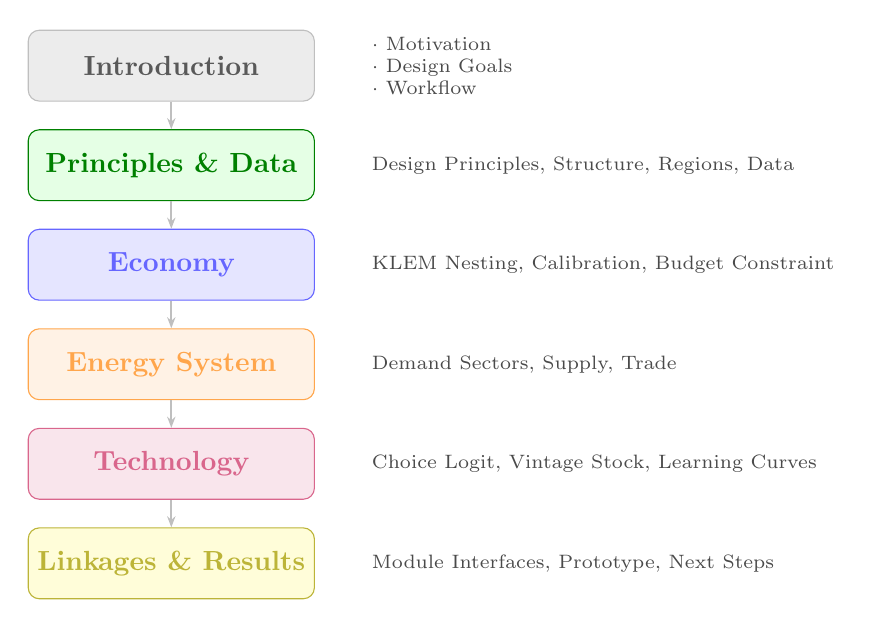
\begin{tikzpicture}[
  box/.style={rounded corners=4pt, minimum width=3.4cm, minimum height=0.9cm,
              align=center, font=\normalsize\bfseries, text width=3.4cm},
  sub/.style={font=\scriptsize, text=TextGray, anchor=west},
  arr/.style={-{Stealth[length=4pt]}, gray!50, thick},
  node distance=0.35cm,
]
  \node[box, fill=gray!15,     draw=gray!50,   text=gray!70!black]                  (s1) {Introduction};
  \node[box, fill=green!10,    draw=green!50!black, text=green!50!black, below=of s1] (s2) {Principles \& Data};
  \node[box, fill=blue!10,     draw=blue!60,   text=blue!60,  below=of s2]           (s3) {Economy};
  \node[box, fill=orange!10,   draw=orange!70, text=orange!70, below=of s3]           (s4) {Energy System};
  \node[box, fill=purple!10,   draw=purple!60, text=purple!60, below=of s4]           (s5) {Technology};
  \node[box, fill=yellow!15,   draw=yellow!70!black, text=yellow!70!black, below=of s5] (s6) {Linkages \& Results};

  \node[sub, right=0.6cm of s1, align=left] {$\cdot$ Motivation\\ $\cdot$ Design Goals\\ $\cdot$ Workflow};
  \node[sub, right=0.6cm of s2] {Design Principles, Structure, Regions, Data};
  \node[sub, right=0.6cm of s3] {KLEM Nesting, Calibration, Budget Constraint};
  \node[sub, right=0.6cm of s4] {Demand Sectors, Supply, Trade};
  \node[sub, right=0.6cm of s5] {Choice Logit, Vintage Stock, Learning Curves};
  \node[sub, right=0.6cm of s6] {Module Interfaces, Prototype, Next Steps};

  \draw[arr] (s1) -- (s2);
  \draw[arr] (s2) -- (s3);
  \draw[arr] (s3) -- (s4);
  \draw[arr] (s4) -- (s5);
  \draw[arr] (s5) -- (s6);
\end{tikzpicture}
\end{frame}

% ══════════════════════════════════════════════════════════════════
\section{Introduction}
% ══════════════════════════════════════════════════════════════════

% ── Slide 3: Motivation — Before / GHIM ──────────────────────────
\begin{frame}{Motivation: What GHIM Brings}
\vspace{1.5em}
\centering
\footnotesize
\renewcommand{\arraystretch}{2.4}
\begin{tabular}{@{} l l l @{}}
\toprule
& \textbf{Before} & \textbf{GHIM} \\
\midrule
\rowcolor{blue!6}
\textbf{\color{blue!60}Economy}
  & More energy detail, less macro feedback
  & Energy $\leftrightarrow$ production feedback (KLEM) \\
\textbf{\color{red!60!black}Climate}
  & Soft coupling or one-way feedback
  & Two-way coupling with multiple channels \\
\rowcolor{purple!6}
\textbf{\color{purple!60}Technology}
  & Mostly fixed cost assumptions
  & Two-factor learning: technology-specific RND + LBD \\
\rowcolor{green!6}
\textbf{\color{green!50!black}Resolution}
  & $\sim$32 regions, 5-year timesteps
  & 100+ countries, annual resolution \\
\textbf{\color{orange!70!black}Solution}
  & Solve one period at a time (no foresight)
  & Adjustable rolling foresight \\
\rowcolor{cyan!6}
\textbf{\color{cyan!60!black}Reporting}
  & Post-hoc translation for IPCC
  & Direct AR6 IAMC-format output \\
\bottomrule
\end{tabular}
\end{frame}

% ── Slide 4: Design Goals ─────────────────────────────────────────
\begin{frame}{Design Goals}
\begin{columns}[T]
\column{0.48\textwidth}
\begin{tcolorbox}[goalbox, colback=blue!8, colframe=blue!60, title={\color{white}1\quad Replicates SSP Baselines}]
\scriptsize Reproduces SSP trajectories before layering policy.
\end{tcolorbox}
\vspace{0.15em}
\begin{tcolorbox}[goalbox, colback=orange!8, colframe=orange!70!black, title={\color{white}3\quad Solve Less, Simulate More}]
\scriptsize Logit-based design for robust convergence.
\end{tcolorbox}
\vspace{0.15em}
\begin{tcolorbox}[goalbox, colback=indigo!8, colframe=indigo!60, title={\color{white}5\quad Transparent \& Reproducible}]
\scriptsize Open-source, every parameter traceable to raw data.
\end{tcolorbox}
\vspace{0.15em}
\begin{tcolorbox}[goalbox, colback=teal!8, colframe=teal!60, title={\color{white}7\quad Open Economy}]
\scriptsize Global market clearing for key commodities.
\end{tcolorbox}

\column{0.48\textwidth}
\begin{tcolorbox}[goalbox, colback=green!8, colframe=green!50!black, title={\color{white}2\quad Hard-couple Energy and Economy}]
\scriptsize KLEM production with native energy accounting.
\end{tcolorbox}
\vspace{0.15em}
\begin{tcolorbox}[goalbox, colback=purple!8, colframe=purple!60, title={\color{white}4\quad IAMC-Native Reporting}]
\scriptsize Model structure mirrors IAMC reporting.
\end{tcolorbox}
\vspace{0.15em}
\begin{tcolorbox}[goalbox, colback=yellow!12, colframe=yellow!70!black, title={\color{white}6\quad User-Configurable}]
\scriptsize Easy to adjust resolution, nesting, sector structure.
\end{tcolorbox}
\vspace{0.15em}
\begin{tcolorbox}[goalbox, colback=red!8, colframe=red!50!black, title={\color{white}8\quad Module Linkage}]
\scriptsize Defined interfaces for other GHIM modules.
\end{tcolorbox}
\end{columns}
\end{frame}

% ── Slide 5: Model Workflow ──────────────────────────────────────
\begin{frame}{Model Workflow}
\centering
\begin{tikzpicture}[
  bigbox/.style={draw=SpruceGreen, thick, rounded corners=2pt, fill=green!5,
                 minimum width=3cm, minimum height=1.5cm, align=center,
                 font=\bfseries\color{TextDark}},
  arr/.style={-{Stealth[length=10pt, width=8pt]}, SpruceGreen, line width=2.5pt},
]
  % Fix bounding box across all overlays
  \useasboundingbox (-7.2, -2.8) rectangle (7.5, 2.8);
  % ── All nodes defined first ──
  % ── All three dotted boxes: exactly 4.6cm × 4.2cm ──
  % Dotted box shells (fixed size, all identical)
  \node<1->[draw=TextLight, dotted, thick, rounded corners=3pt,
        minimum height=4.6cm, minimum width=3.8cm] (gcambox) at (-5.2, 0) {};
  \node<2->[draw=TextLight, dotted, thick, rounded corners=3pt,
        minimum height=4.6cm, minimum width=3.8cm] (ghimbox) at (0, 0) {};
  \node<3->[draw=TextLight, dotted, thick, rounded corners=3pt,
        minimum height=4.6cm, minimum width=3.8cm] (iamcbox) at (5.2, 0) {};

  % gcamdata contents
  \node<1->[inner sep=0] (gcam) at (-5.2, 0.3) {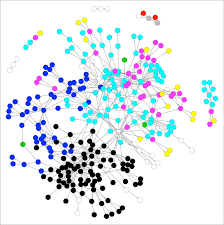
\includegraphics[width=2.4cm]{gcamdata.png}};
  \node<1->[below=1pt of gcam, font=\small\color{TextGray}] (gcamlabel) {gcamdata input};
  \node<1->[below=1pt of gcamlabel, font=\tiny\color{TextLight}, align=center, text width=3.0cm] (sources) {SSP $\cdot$ IEA $\cdot$ UN $\cdot$ FAO $\cdot$ CEDS\\NREL $\cdot$ GTAP $\cdot$ USGS $\cdot$ EDGAR};

  % GHIM contents
  \node<2->[bigbox, minimum width=2.8cm, minimum height=1.2cm, font=\small\bfseries\color{TextDark}] (ghim) at (0, 1.0) {GHIM\\Energy Module};
  \node<2->[draw=SpruceGreen, dashed, thick, rounded corners=2pt, fill=green!5,
        minimum width=2.8cm, minimum height=1.2cm, align=center,
        font=\small\bfseries\color{TextDark}] (other) at (0, -1.0) {GHIM\\Other Modules};
  \draw<2->[{Stealth[length=6pt, width=5pt]}-{Stealth[length=6pt, width=5pt]}, SpruceGreen, line width=1.5pt] ([yshift=-4pt]ghim.south) -- ([yshift=4pt]other.north);

  % IAMC contents
  \node<3->[inner sep=0] (iamc) at (5.2, 0.2) {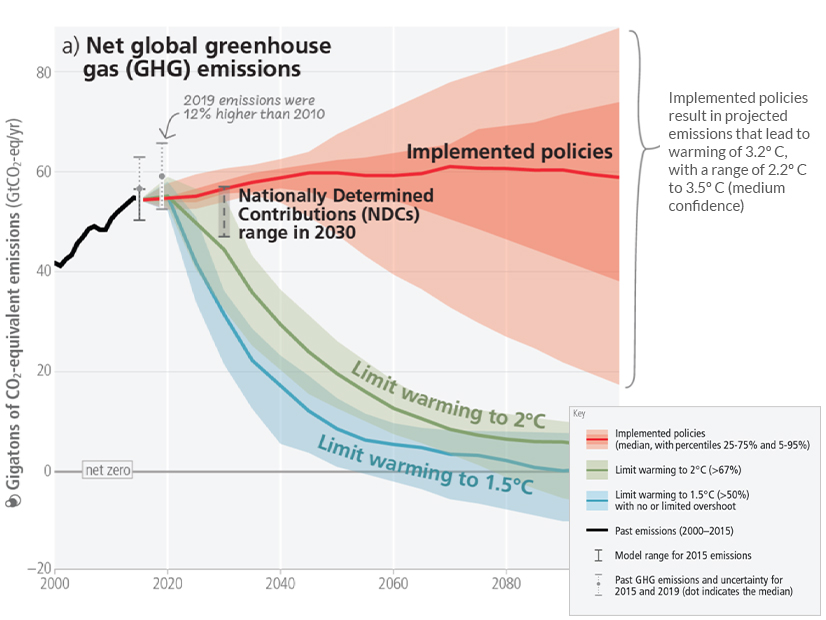
\includegraphics[width=2.8cm]{iamc.jpeg}};
  \node<3->[below=3pt of iamc, font=\small\color{TextGray}] (iamclabel) {IAMC data template};

  % ── Arrows (reference nodes defined above) ──
  \draw<2->[arr] ([xshift=6pt]gcambox.east) -- ([xshift=-6pt]ghimbox.west);
  \draw<3->[arr] ([xshift=6pt]ghimbox.east) -- ([xshift=-6pt]iamcbox.west);
\end{tikzpicture}
\end{frame}

% ══════════════════════════════════════════════════════════════════
\section{Framework \& Data}
% ══════════════════════════════════════════════════════════════════

% ── Slide 6: General Model Structure by Phase ────────────────────
\begin{frame}{General Model Structure by Phase}
\centering
\footnotesize
\begin{tabular}{l p{5.2cm} p{5.2cm}}
\toprule
\textbf{Component} & \textbf{Phase 1} & \textbf{Phase 2} \\
\midrule
\rowcolor{SpruceGreen!8}
Time          & 2000--2150, 5-year steps              & Annual resolution \\
Region        & 32 Regions                 & 100+ countries \\
\rowcolor{SpruceGreen!8}
Economy       & GDP $= f$(Capital, Labor, Energy, Materials) & + Energy intensity $EI = f(\mathrm{RND})$ \\
Solution      & Recursive-dynamic                      & Adjustable rolling foresight \\
\rowcolor{SpruceGreen!8}
Energy System & Minimum nesting for AR6 Tier-1         & Expanded nesting for Tier-3 \\
Trade         & Global fossil fuel market clearing      & Multi-commodity global trade \\
Coupling      & One-way coupling with Land              & Two-way with multiple modules \\
\midrule
\rowcolor{SpruceGreen!8}
\multicolumn{1}{l}{Tech.\ Choice} & \multicolumn{2}{p{10.0cm}}{Absolute cost logit with SSP-calibrated preference weights} \\
\multicolumn{1}{l}{Tech.\ Change} & \multicolumn{2}{p{10.0cm}}{Two-factor learning: RND knowledge + cumulative deployment (LBD)} \\
\bottomrule
\end{tabular}
\end{frame}

% ── Slide 7: Regional Classification ─────────────────────────────
\begin{frame}{32 Regions of Phase 1}
\centering
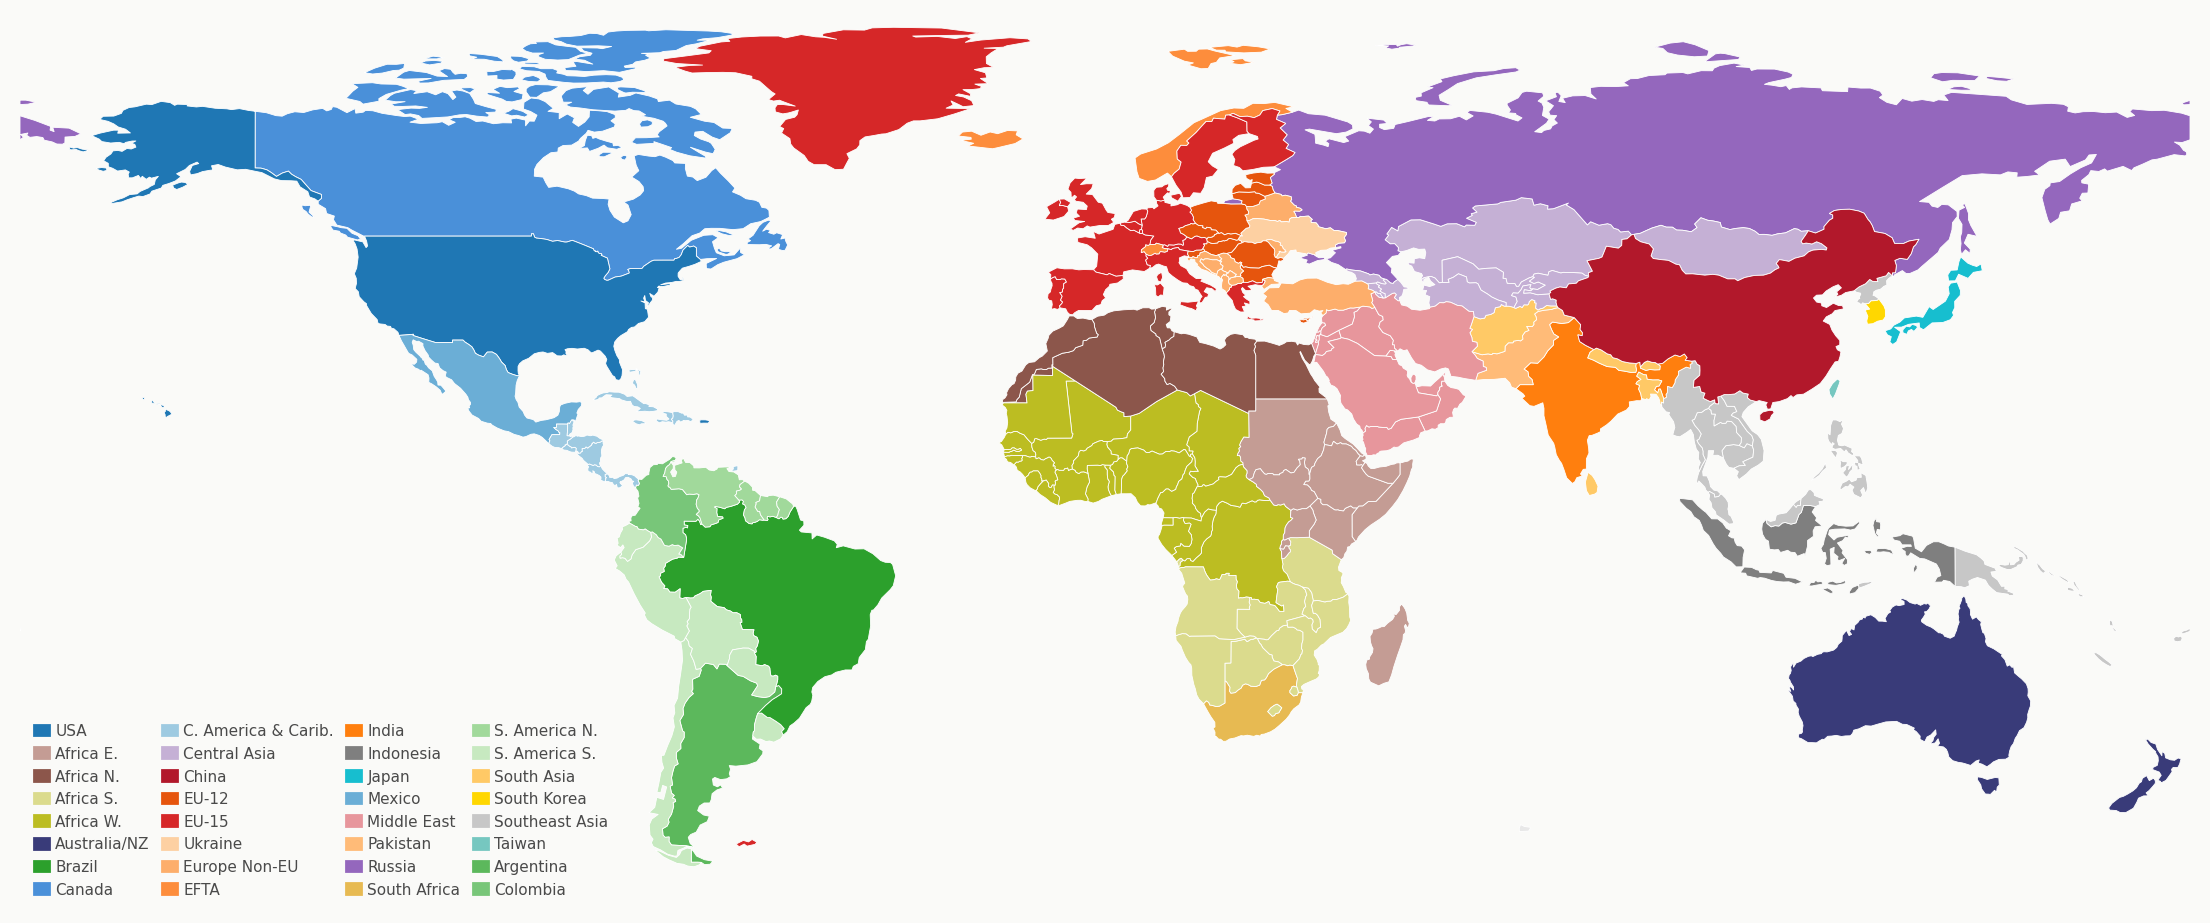
\includegraphics[width=\linewidth, height=0.78\textheight, keepaspectratio]{r32_world_map.png}
\end{frame}

% ── Slide 8: Model Overview (animated) ──────────────────────────
\begin{frame}{Model Overview}
\centering
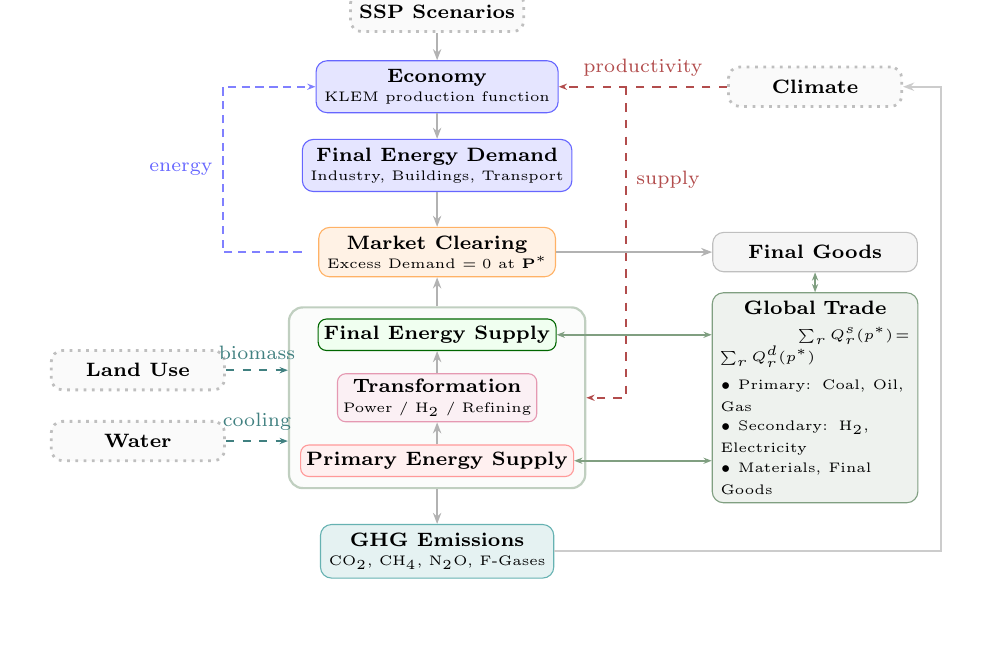
\begin{tikzpicture}[
  mbox/.style={rounded corners=4pt, minimum width=2.4cm, minimum height=0.5cm,
               align=center, font=\scriptsize, inner sep=3pt},
  sbox/.style={rounded corners=3pt, minimum width=2.2cm, minimum height=0.4cm,
               align=center, font=\scriptsize, inner sep=2pt},
  outer/.style={rounded corners=4pt, draw=gray!50, dotted, line width=1pt,
               fill=gray!4, minimum width=2.2cm, minimum height=0.5cm,
               align=center, font=\scriptsize, inner sep=3pt},
  pbox/.style={rounded corners=5pt, draw=SpruceGreen!30, line width=0.8pt,
               inner sep=4pt, fill=SpruceGreen!2},
  arr/.style={-{Stealth[length=4pt]}, gray!60, thick},
  fb/.style={-{Stealth[length=3pt]}, red!40!gray, thick, dashed},
  price/.style={-{Stealth[length=3pt]}, blue!50, thick, densely dashed},
  ext/.style={-{Stealth[length=3pt]}, teal!50!gray, thick, dashed},
  trade/.style={{Stealth[length=3pt]}-{Stealth[length=3pt]}, SpruceGreen!60, thick},
]
  % Fix bounding box so elements don't shift during animation
  \useasboundingbox (-5.2, -7.3) rectangle (6.8, 0.5);

  % ═══ Step 1: SSP ═══
  \node<1->[outer] (ssp) at (0, 0.7)
    {\textbf{SSP Scenarios}};

  % ═══ Step 2: Economy ═══
  \node<2->[mbox, fill=blue!10, draw=blue!60] (econ) at (0, -0.25)
    {\textbf{Economy}\\[-1pt]{\tiny KLEM production function}};
  \draw<2->[arr] (ssp) -- (econ);

  % ═══ Step 3: Final Energy Demand ═══
  \node<3->[mbox, fill=blue!10, draw=blue!60] (fed) at (0, -1.25)
    {\textbf{Final Energy Demand}\\[-1pt]{\tiny Industry, Buildings, Transport}};
  \draw<3->[arr] (econ) -- (fed);

  % ═══ Step 4: Primary Energy Supply ═══
  \node<4->[sbox, fill=red!6, draw=red!40] (pes) at (0, -5.0)
    {\textbf{Primary Energy Supply}};

  % ═══ Step 5: Transformation ═══
  \node<5->[sbox, fill=purple!6, draw=purple!40] (trans) at (0, -4.2)
    {\textbf{Transformation}\\[-1pt]{\tiny Power / H$_2$ / Refining}};
  \draw<5->[arr] (pes) -- (trans);

  % ═══ Step 6: FES + prod group + Land Use / Water ═══
  \node<6->[sbox, fill=green!6, draw=green!40!black] (fes) at (0, -3.4)
    {\textbf{Final Energy Supply}};
  \draw<6->[arr] (trans) -- (fes);
  \begin{scope}[on background layer]
    \node<6->[pbox, fit=(pes)(trans)(fes)] (prod) {};
  \end{scope}
  \node<6->[outer] (land) at (-3.8, -3.85)
    {\textbf{Land Use}};
  \node<6->[outer] (water) at (-3.8, -4.75)
    {\textbf{Water}};
  \draw<6->[ext] (land) -- node[above, font=\scriptsize, text=teal!50!gray] {biomass} (land -| prod.west);
  \draw<6->[ext] (water) -- node[above, font=\scriptsize, text=teal!50!gray] {cooling} (water -| prod.west);

  % ═══ Step 7: Market Clearing ═══
  \node<7->[mbox, fill=orange!10, draw=orange!60] (emc) at (0, -2.35)
    {\textbf{Market Clearing}\\[-1pt]{\tiny Excess Demand $= 0$ at $\mathbf{P}^*$}};
  \draw<7->[arr] (fed) -- (emc);
  \draw<7->[arr] (prod.north) -- (emc);

  % ═══ Step 8: Final Goods + energy feedback ═══
  \node<8->[mbox, fill=gray!8, draw=gray!50, minimum width=2.6cm] (fgs) at (4.8, -2.35)
    {\textbf{Final Goods}};
  \draw<8->[arr] (emc) -- (fgs);
  \draw<8->[price] ([xshift=-6pt]emc.west) -- ++(-1.0, 0)
    |- node[pos=0.25, left, font=\scriptsize, text=blue!60] {energy} (econ.west);

  % ═══ Step 9: Global Trade + trade arrows ═══
  \node<9->[mbox, fill=SpruceGreen!8, draw=SpruceGreen!60,
        minimum height=2.2cm, text width=2.4cm, align=left] (gtrade) at (4.8, -4.2)
    {\hfil\textbf{Global Trade}\hfil\\[1pt]
     \hfil{\tiny $\sum_r Q^s_r(p^*)\!=\!\sum_r Q^d_r(p^*)$}\hfil\\[2pt]
     {\tiny$\bullet$ Primary: Coal, Oil, Gas}\\[-1pt]
     {\tiny$\bullet$ Secondary: H$_2$, Electricity}\\[-1pt]
     {\tiny$\bullet$ Materials, Final Goods}};
  \draw<9->[trade] (pes.east) -- (pes -| gtrade.west);
  \draw<9->[trade] (fes.east) -- (fes -| gtrade.west);
  \draw<9->[trade] (fgs.south) -- (gtrade.north);

  % ═══ Step 10: GHG Emissions ═══
  \node<10->[mbox, fill=teal!10, draw=teal!60] (emis) at (0, -6.15)
    {\textbf{GHG Emissions}\\[-1pt]{\tiny CO$_2$, CH$_4$, N$_2$O, F-Gases}};
  \draw<10->[arr] (prod.south) -- (emis);

  % ═══ Step 11: Climate + productivity / supply feedbacks ═══
  \node<11->[outer] (climate) at (4.8, -0.25)
    {\textbf{Climate}};
  \draw<11->[arr, gray!40] (emis.east) -- (6.4, -6.15)
    -- (6.4, -0.25) -- (climate.east);
  \draw<11->[fb] (climate.west) -- node[above, font=\scriptsize, text=red!40!gray, midway] {productivity} (econ.east);
  \draw<11->[fb] (2.4, -0.25) -- node[right, font=\scriptsize, text=red!40!gray, pos=0.3] {supply}
    (2.4, -4.2) -- (prod.east);
\end{tikzpicture}
\end{frame}

% ── Slide 8b: Model Overview (static, white, no title) ──────────
{%
\setbeamercolor{background canvas}{bg=white}
\begin{frame}[plain]
\centering
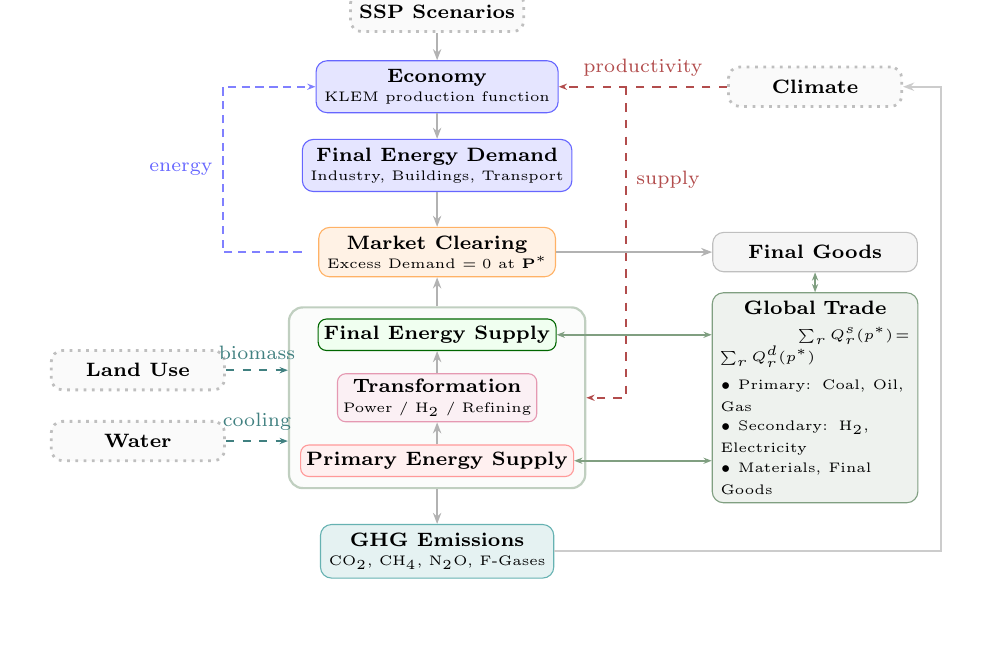
\begin{tikzpicture}[
  mbox/.style={rounded corners=4pt, minimum width=2.4cm, minimum height=0.5cm,
               align=center, font=\scriptsize, inner sep=3pt},
  sbox/.style={rounded corners=3pt, minimum width=2.2cm, minimum height=0.4cm,
               align=center, font=\scriptsize, inner sep=2pt},
  outer/.style={rounded corners=4pt, draw=gray!50, dotted, line width=1pt,
               fill=gray!4, minimum width=2.2cm, minimum height=0.5cm,
               align=center, font=\scriptsize, inner sep=3pt},
  pbox/.style={rounded corners=5pt, draw=SpruceGreen!30, line width=0.8pt,
               inner sep=4pt, fill=SpruceGreen!2},
  arr/.style={-{Stealth[length=4pt]}, gray!60, thick},
  fb/.style={-{Stealth[length=3pt]}, red!40!gray, thick, dashed},
  price/.style={-{Stealth[length=3pt]}, blue!50, thick, densely dashed},
  ext/.style={-{Stealth[length=3pt]}, teal!50!gray, thick, dashed},
  trade/.style={{Stealth[length=3pt]}-{Stealth[length=3pt]}, SpruceGreen!60, thick},
]
  \useasboundingbox (-5.2, -7.3) rectangle (6.8, 0.5);

  \node[outer] (ssp) at (0, 0.7) {\textbf{SSP Scenarios}};
  \node[mbox, fill=blue!10, draw=blue!60] (econ) at (0, -0.25)
    {\textbf{Economy}\\[-1pt]{\tiny KLEM production function}};
  \draw[arr] (ssp) -- (econ);
  \node[mbox, fill=blue!10, draw=blue!60] (fed) at (0, -1.25)
    {\textbf{Final Energy Demand}\\[-1pt]{\tiny Industry, Buildings, Transport}};
  \draw[arr] (econ) -- (fed);
  \node[sbox, fill=red!6, draw=red!40] (pes) at (0, -5.0)
    {\textbf{Primary Energy Supply}};
  \node[sbox, fill=purple!6, draw=purple!40] (trans) at (0, -4.2)
    {\textbf{Transformation}\\[-1pt]{\tiny Power / H$_2$ / Refining}};
  \draw[arr] (pes) -- (trans);
  \node[sbox, fill=green!6, draw=green!40!black] (fes) at (0, -3.4)
    {\textbf{Final Energy Supply}};
  \draw[arr] (trans) -- (fes);
  \begin{scope}[on background layer]
    \node[pbox, fit=(pes)(trans)(fes)] (prod) {};
  \end{scope}
  \node[outer] (land) at (-3.8, -3.85) {\textbf{Land Use}};
  \node[outer] (water) at (-3.8, -4.75) {\textbf{Water}};
  \draw[ext] (land) -- node[above, font=\scriptsize, text=teal!50!gray] {biomass} (land -| prod.west);
  \draw[ext] (water) -- node[above, font=\scriptsize, text=teal!50!gray] {cooling} (water -| prod.west);
  \node[mbox, fill=orange!10, draw=orange!60] (emc) at (0, -2.35)
    {\textbf{Market Clearing}\\[-1pt]{\tiny Excess Demand $= 0$ at $\mathbf{P}^*$}};
  \draw[arr] (fed) -- (emc);
  \draw[arr] (prod.north) -- (emc);
  \node[mbox, fill=gray!8, draw=gray!50, minimum width=2.6cm] (fgs) at (4.8, -2.35)
    {\textbf{Final Goods}};
  \draw[arr] (emc) -- (fgs);
  \draw[price] ([xshift=-6pt]emc.west) -- ++(-1.0, 0)
    |- node[pos=0.25, left, font=\scriptsize, text=blue!60] {energy} (econ.west);
  \node[mbox, fill=SpruceGreen!8, draw=SpruceGreen!60,
        minimum height=2.2cm, text width=2.4cm, align=left] (gtrade) at (4.8, -4.2)
    {\hfil\textbf{Global Trade}\hfil\\[1pt]
     \hfil{\tiny $\sum_r Q^s_r(p^*)\!=\!\sum_r Q^d_r(p^*)$}\hfil\\[2pt]
     {\tiny$\bullet$ Primary: Coal, Oil, Gas}\\[-1pt]
     {\tiny$\bullet$ Secondary: H$_2$, Electricity}\\[-1pt]
     {\tiny$\bullet$ Materials, Final Goods}};
  \draw[trade] (pes.east) -- (pes -| gtrade.west);
  \draw[trade] (fes.east) -- (fes -| gtrade.west);
  \draw[trade] (fgs.south) -- (gtrade.north);
  \node[mbox, fill=teal!10, draw=teal!60] (emis) at (0, -6.15)
    {\textbf{GHG Emissions}\\[-1pt]{\tiny CO$_2$, CH$_4$, N$_2$O, F-Gases}};
  \draw[arr] (prod.south) -- (emis);
  \node[outer] (climate) at (4.8, -0.25) {\textbf{Climate}};
  \draw[arr, gray!40] (emis.east) -- (6.4, -6.15) -- (6.4, -0.25) -- (climate.east);
  \draw[fb] (climate.west) -- node[above, font=\scriptsize, text=red!40!gray, midway] {productivity} (econ.east);
  \draw[fb] (2.4, -0.25) -- node[right, font=\scriptsize, text=red!40!gray, pos=0.3] {supply}
    (2.4, -4.2) -- (prod.east);
\end{tikzpicture}
\end{frame}
}%

% ── Slide 9: Input Data ──────────────────────────────────────────
\begin{frame}{Input Data: The GCAM Data System}
\begin{columns}[T]
  \begin{column}{0.42\textwidth}
    \centering
    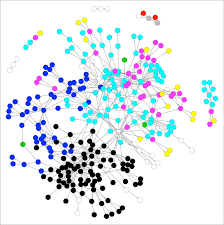
\includegraphics[width=\linewidth, height=0.7\textheight, keepaspectratio]{gcamdata.png}
  \end{column}
  \begin{column}{0.55\textwidth}
    \small
    \begin{tabular}{@{} l l l @{}}
    \toprule
    \textbf{Category} & \textbf{Source} & \textbf{Version} \\
    \midrule
    \rowcolor{SpruceGreen!8}
    Energy balances & IEA WEB & 2023 \\
    Scenarios & IIASA SSP & AR6 \\
    \rowcolor{SpruceGreen!8}
    Emissions & CEDS & 2022 \\
    \rowcolor{SpruceGreen!8}
    Trade & GTAP & v11 \\
    Resources & NREL ATB & 2024 \\
    \rowcolor{SpruceGreen!8}
    Transport & UCD & 2013 \\
    Land / Agriculture & FAO & 2024 \\
    \bottomrule
    \end{tabular}

    \vspace{0.3em}
    {\tiny\color{TextLight}%
    \begin{tabular}[t]{@{$\bullet$\;}l@{}}
    IEA: International Energy Agency\\
    CEDS: Community Emissions Data System\\
    GTAP: Global Trade Analysis Project\\
    NREL: National Renewable Energy Lab\\
    UCD: UC Davis Transportation Database\\
    FAO: Food \& Agriculture Organization
    \end{tabular}}
  \end{column}
\end{columns}
\end{frame}

% ── Slide 9b: Data Pipeline ──────────────────────────────────────
\begin{frame}[t]{Data Pipeline: From Sources to Model Objects}

\begin{columns}[T]
\column{0.48\textwidth}

{\small\bfseries\color{SpruceGreen} Channel 1: Calibration Targets}

\vspace{0.6em}

\centering
\scalebox{0.88}{
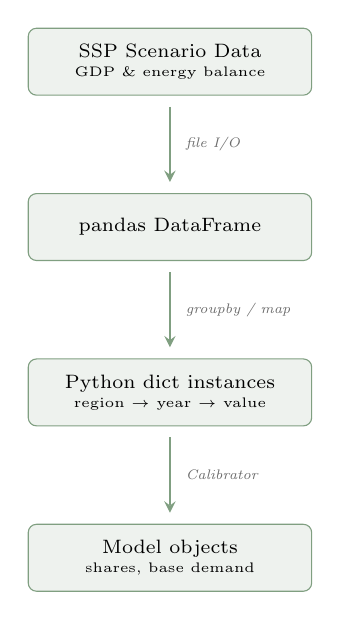
\begin{tikzpicture}[
  box/.style={rounded corners=3pt, draw=SpruceGreen!60, fill=SpruceGreen!8,
              minimum width=3.6cm, minimum height=0.85cm, font=\scriptsize,
              align=center, inner sep=5pt},
  arr/.style={->, >=stealth, thick, SpruceGreen!60, shorten <=4pt, shorten >=4pt},
  lbl/.style={font=\tiny\itshape, text=TextLight},
]
  \node[box] (ssp) at (0,0) {SSP Scenario Data\\[-1pt]{\tiny GDP \& energy balance}};
  \node[box] (df)  at (0,-2.1) {pandas DataFrame};
  \node[box] (dict) at (0,-4.2) {Python dict instances\\[-1pt]{\tiny region $\to$ year $\to$ value}};
  \node[box] (obj) at (0,-6.3) {Model objects\\[-1pt]{\tiny shares, base demand}};

  \draw[arr] (ssp)  -- (df)   node[lbl, midway, right, xshift=2pt] {file I/O};
  \draw[arr] (df)   -- (dict) node[lbl, midway, right, xshift=2pt] {groupby / map};
  \draw[arr] (dict) -- (obj)  node[lbl, midway, right, xshift=2pt] {Calibrator};
\end{tikzpicture}
}

\column{0.48\textwidth}

{\small\bfseries\color{SpruceGreen} Channel 2: Structural Parameters}

\vspace{0.6em}

\centering
\scalebox{0.88}{
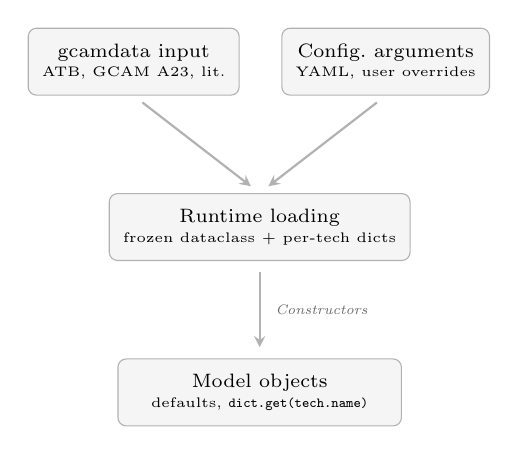
\begin{tikzpicture}[
  box/.style={rounded corners=3pt, draw=gray!60, fill=gray!8,
              minimum width=2.6cm, minimum height=0.85cm, font=\scriptsize,
              align=center, inner sep=5pt},
  wide/.style={box, minimum width=3.6cm},
  arr/.style={->, >=stealth, thick, gray!60, shorten <=4pt, shorten >=4pt},
  lbl/.style={font=\tiny\itshape, text=TextLight},
]
  \node[box] (gcam) at (-1.6,0) {gcamdata input\\[-1pt]{\tiny ATB, GCAM A23, lit.}};
  \node[box] (args) at (1.6,0) {Config.\ arguments\\[-1pt]{\tiny YAML, user overrides}};
  \node[wide] (load) at (0,-2.1) {Runtime loading\\[-1pt]{\tiny frozen dataclass + per-tech dicts}};
  \node[wide] (obj) at (0,-4.2) {Model objects\\[-1pt]{\tiny defaults, \texttt{dict.get(tech.name)}}};

  \draw[arr] (gcam.south) -- (load.north);
  \draw[arr] (args.south) -- (load.north);
  \draw[arr] (load) -- (obj)  node[lbl, midway, right, xshift=2pt] {Constructors};
\end{tikzpicture}
}

\end{columns}

\end{frame}

% ══════════════════════════════════════════════════════════════════
\section{Economy}
% ══════════════════════════════════════════════════════════════════

% ── Slide 10: KLEM Economy — Phase 1 Design ───────────────────
\begin{frame}[t]{KLEM Economy --- Phase 1 Design}
\begin{columns}[T]
\column{0.42\textwidth}
\centering
{\small\bfseries Nesting Structure}

\vspace{0.2em}
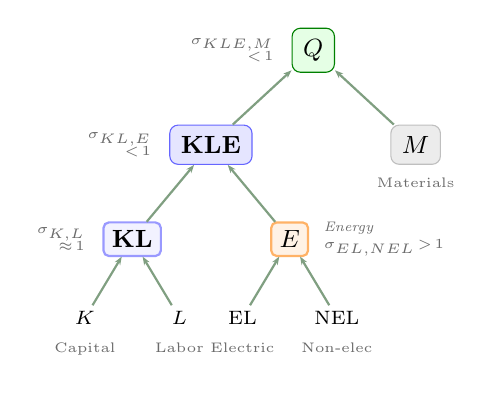
\begin{tikzpicture}[
  nd/.style={font=\small\bfseries, inner sep=2pt},
  lbl/.style={font=\tiny\itshape, text=TextLight},
  edge from parent/.style={draw=SpruceGreen!60, thick, {Stealth[length=3pt]}-},
  level 1/.style={sibling distance=2.6cm, level distance=1.2cm},
  level 2/.style={sibling distance=2.0cm, level distance=1.2cm},
  level 3/.style={sibling distance=1.2cm, level distance=1.0cm},
]
  \node[nd, fill=green!10, draw=green!50!black, rounded corners=3pt, inner sep=4pt] (Q) {$Q$}
    child {
      node[nd, fill=blue!10, draw=blue!60, rounded corners=3pt, inner sep=4pt] (KLE) {KLE}
        child {
          node[nd, fill=blue!5, draw=blue!40, rounded corners=2pt, inner sep=3pt] (KL) {KL}
            child { node[nd, font=\scriptsize] (Kn) {$K$} }
            child { node[nd, font=\scriptsize] (Ln) {$L$} }
        }
        child {
          node[nd, fill=orange!10, draw=orange!60, rounded corners=2pt, inner sep=3pt] (E) {$E$}
            child { node[nd, font=\scriptsize] (ELn) {EL} }
            child { node[nd, font=\scriptsize] (NELn) {NEL} }
        }
    }
    child {
      node[nd, fill=gray!15, draw=gray!50, rounded corners=3pt, inner sep=4pt] (M) {$M$}
    };
  % Leaf labels
  \node[font=\tiny, text=TextLight, below=1pt of Kn] {Capital};
  \node[font=\tiny, text=TextLight, below=1pt of Ln] {Labor};
  \node[font=\tiny, text=TextLight, below=1pt of ELn] {Electric};
  \node[font=\tiny, text=TextLight, below=1pt of NELn] {Non-elec};
  \node[font=\tiny, text=TextLight, below=1pt of M] {Materials};
  % CES labels
  \node[lbl, left=3pt of Q, align=right] {$\sigma_{KLE,M}$\\$<\!1$};
  \node[lbl, left=3pt of KLE, align=right] {$\sigma_{KL,E}$\\$<\!1$};
  \node[lbl, left=1pt of KL, xshift=-2pt, align=right] {$\sigma_{K,L}$\\$\approx\!1$};
  \node[lbl, right=2pt of E, align=left] {Energy\\$\sigma_{EL,NEL}\!>\!1$};
  %\node[lbl, right=2pt of M] {exog.};
\end{tikzpicture}

\vspace{0.3em}
{\tiny\color{TextLight}\raggedright%
\begin{tabular}[t]{@{$\bullet$\;}l@{}}
CES: Constant Elasticity of Substitution\\
Each nest has its own $\sigma$ $\to$ heterogeneous substitution\\
$\sigma\!<\!1$: complements;\; $\sigma\!>\!1$: substitutes\\
$\sigma\!\approx\!1$: unit elastic (Cobb-Douglas)
\end{tabular}}

\vspace{0.1em}
\column{0.55\textwidth}
\visible<2->{%
\begin{tcolorbox}[infobox, colback=green!6, colframe=green!50!black, title=Key Equations, top=2pt, bottom=2pt]
\small
\textbf{Gross Output:}\quad $Q = \mathrm{CES}(KLE,\; M)$

\vspace{1pt}
\textbf{Net output (=GDP):}\quad $Y = Q - p_E \!\cdot\! E - p_M \!\cdot\! M$

\vspace{1pt}
\textbf{Factor services:}\quad $KL = \mathrm{CES}(K,\; L;\; \sigma_{K,L})$

\vspace{1pt}
\textbf{Energy demand:}\quad {\scriptsize $E = E_0 \!\cdot\! \frac{KL}{KL_0} \!\cdot\! \bigl(\frac{p_E}{p_{E,0}}\bigr)^{-\sigma_{KL,E}}$}

\vspace{1pt}
\textbf{Budget:}\quad $I_K = s \!\cdot\! Y - I_{energy} - \sum_j I_{RD,j}$
\end{tcolorbox}}

\vspace{0.1em}
\visible<3->{%
\begin{tcolorbox}[infobox, colback=yellow!6, colframe=yellow!60!black, title=Feedback Mechanisms, top=2pt, bottom=2pt]
\small
$\bullet$~$p_E \!\uparrow\;\Rightarrow\; E\!\downarrow\;\Rightarrow\; Q\!\downarrow\;\Rightarrow\; Y\!\downarrow$

\smallskip
$\bullet$~$\sigma_{EL,NEL}\!>\!1$: electric $\leftrightarrow$ fossil substitutable\\
\phantom{$\bullet$~}$\to$ electrification absorbs fossil price shock\\
\phantom{$\bullet$~}$\to$ lower GDP cost of decarbonization
\end{tcolorbox}}
\end{columns}
\end{frame}

% ── Slide 11: Phase 2 — Energy Services Nest (RDEN) ─────────────
\begin{frame}{Phase 2 --- Energy Services Nest (Aggregate Energy Efficiency Improvement)}
\begin{columns}[T]
\column{0.42\textwidth}
{\small\bfseries Phase 1 $\to$ Phase 2}

\vspace{0.3em}
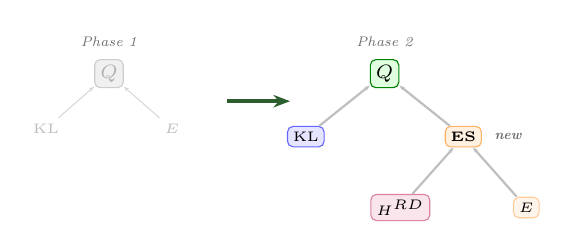
\begin{tikzpicture}[
  nd/.style={font=\scriptsize\bfseries, inner sep=2pt, rounded corners=2pt},
  lbl/.style={font=\tiny\itshape, text=TextLight},
  arr/.style={draw=gray!50, thick, {Stealth[length=2pt]}-},
]
  % Phase 1 (compact, grayed)
  \node[nd, fill=gray!12, draw=gray!40, text=gray!60] (q1) at (0, 0) {$Q$};
  \node[nd, text=gray!50, font=\tiny] (kl1) at (-0.8, -0.7) {KL};
  \node[nd, text=gray!50, font=\tiny] (e1) at (0.8, -0.7) {$E$};
  \draw[draw=gray!30, {Stealth[length=2pt]}-] (q1) -- (kl1);
  \draw[draw=gray!30, {Stealth[length=2pt]}-] (q1) -- (e1);
  \node[lbl, above=1pt of q1] {Phase 1};

  % Arrow
  \draw[-{Stealth[length=6pt]}, SpruceGreen, line width=1.5pt] (1.5, -0.35) -- (2.3, -0.35);

  % Phase 2 (highlighted)
  \node[nd, fill=green!12, draw=green!50!black] (q2) at (3.5, 0) {$Q$};
  \node[nd, fill=blue!10, draw=blue!60, font=\tiny] (kl2) at (2.5, -0.8) {KL};
  \node[nd, fill=orange!12, draw=orange!60, font=\tiny\bfseries] (es) at (4.5, -0.8) {ES};
  \node[nd, fill=purple!10, draw=purple!50, font=\tiny] (hrd) at (3.7, -1.7) {$H^{RD}$};
  \node[nd, fill=orange!8, draw=orange!40, font=\tiny] (e2) at (5.3, -1.7) {$E$};
  \draw[arr] (q2) -- (kl2);
  \draw[arr] (q2) -- (es);
  \draw[arr] (es) -- (hrd);
  \draw[arr] (es) -- (e2);
  \node[lbl, above=1pt of q2] {Phase 2};
  \node[lbl, right=1pt of es] {\textbf{new}};
\end{tikzpicture}

\vspace{0.3em}
{\scriptsize\raggedright%
\begin{tabular}[t]{@{$\bullet$\;}l@{}}
$I_{RD}^{\mathrm{agg}} = s_{RD} \cdot Y$ \quad (GDP fraction)\\
$I_{RD} \to H^{RD}\!\uparrow$ \quad (knowledge stock)\\
$\sigma_{ES}\!>\!1$: $H^{RD}$ substitutes for $E$\\
$E$: EL $+$ NEL (same as Phase 1)\\
$ES = \mathrm{CES}(H^{RD},\; E;\; \sigma_{ES}\!>\!1)$\\[3pt]
\multicolumn{1}{@{}l@{}}{\textit{What is aggregate efficiency?}}\\
Cross-cutting R\&D: insulation, smart grid, \ldots\\
Same output, less energy $\to$ endogenizes AEEI
\end{tabular}}

\column{0.55\textwidth}
\visible<2->{%
\begin{tcolorbox}[infobox, colback=purple!6, colframe=purple!60, title=Energy Service Wraps Physical Energy, top=2pt, bottom=2pt]
\small
Phase 1: $E = ES$ (physical energy $=$ energy service)

\smallskip
$\bullet$~$E$: physical energy input (EJ $\times$ base price)\\
$\bullet$~$H^{RD}$: knowledge stock (R\&D-driven efficiency)\\
$\bullet$~$\sigma_{ES}\!>\!1$: $H^{RD}$ substitutes for $E$

\smallskip
$\to$ Same \textbf{energy services}, less \textbf{physical energy}\\
$\to$ Endogenous energy efficiency improvement
\end{tcolorbox}}

\vspace{0.3em}
\visible<3->{%
\begin{tcolorbox}[infobox, colback=orange!6, colframe=orange!70!black, title=Unified Budget Constraint, top=2pt, bottom=2pt]
\small
$s \cdot Y = I_K + I_{RD}^{\mathrm{agg}} + \sum_j I_{RD,j}$

\smallskip
$\bullet$~More R\&D $\to$ less $K$ short-term\\
\phantom{$\bullet$~}but $H^{RD}\!\uparrow$ $\to$ $E\!\downarrow$ long-term
\end{tcolorbox}}
\end{columns}
\end{frame}

% ── Slide 12: KLEM — Parameter Interpretation ───────────────────
\begin{frame}{KLEM --- Parameter Interpretation}
\vspace{0.2em}
\centering
\small
\begin{tabular}{@{} l l l l @{}}
\toprule
\textbf{Parameter} & \textbf{Value} & \textbf{Nest} & \textbf{Intuition} \\
\midrule
\rowcolor{SpruceGreen!8}
$\sigma_{KL}$ & $\sim$1.0 & KL & Unit elastic (Cobb-Douglas) \\
$\sigma_{KL,E}$ & $\sim$0.4 & KLE & Complements ($<\!1$): energy is essential \\
\rowcolor{SpruceGreen!8}
$\sigma_{EL,NEL}$ & $\sim$2.0 & E & Substitutes ($>\!1$): electric replaces fossil \\
$\sigma_{KLE,M}$ & $\sim$0.5 & Q & Complements ($<\!1$): materials essential \\
\midrule
\rowcolor{SpruceGreen!8}
TFP & calibrated & KL & Matches SSP GDP trajectory \\
$A_{CES}$ & calibrated & CES & Ensures $Y = \text{GDP}$ at base year \\
$s$ & 0.22 & Budget & GDP reinvestment rate \\
\rowcolor{SpruceGreen!8}
$\delta$ & 0.05 & Capital & Annual depreciation rate \\
LFP & regional & Labor & ILO 2020 workforce fraction \\
\bottomrule
\end{tabular}
\end{frame}

% ── Slide 13: Calibration — Matching SSP Trajectories ───────────
\begin{frame}[t]{Calibration --- Matching SSP Trajectories}
\vspace{-0.4em}

\begin{tcolorbox}[infobox, colback=green!6, colframe=green!50!black, top=3pt, bottom=3pt, title={Step 1 --- Input Weights $\alpha$ \quad{\normalfont\scriptsize(base year, time-invariant)}}]
\small Base-year spending fractions on K, L, E, M determine CES weights
\end{tcolorbox}

\vspace{-0.1em}
\begin{tcolorbox}[infobox, colback=blue!6, colframe=blue!60, top=3pt, bottom=3pt, title={Step 2 --- Scale Factors $A$ \quad{\normalfont\scriptsize(base year, time-invariant)}}]
\small Adjust each nest so CES output matches observed base-year values
\end{tcolorbox}

\vspace{-0.1em}
\begin{tcolorbox}[infobox, colback=orange!6, colframe=orange!70!black, top=3pt, bottom=3pt, title=Step 3 --- Productivity TFP$(t)$ \quad{\normalfont\scriptsize(solved at every future year)}]
\small Find TFP$(t)$ so that:\quad $Q(t) - p_E\!\cdot\! E - p_M\!\cdot\! M = \mathrm{GDP}_{\mathrm{SSP}}(t)$
\end{tcolorbox}

\vspace{-0.1em}
\begin{tcolorbox}[enhanced, colback=SpruceGreen!6, colframe=SpruceGreen, boxrule=0.8pt, arc=3pt, left=5pt, right=5pt, top=3pt, bottom=3pt, fonttitle=\small\bfseries, title=Result]
\small Reference run reproduces SSP GDP within tolerance ($< 0.2\%$ deviation).
\end{tcolorbox}
\end{frame}

\section{Energy System}

% ── Slide 11: Energy System Overview ──────────────────────────────
\begin{frame}{Energy System Overview (Phase 1)}
\centering
\pgfdeclarelayer{background}
\pgfsetlayers{background,main}
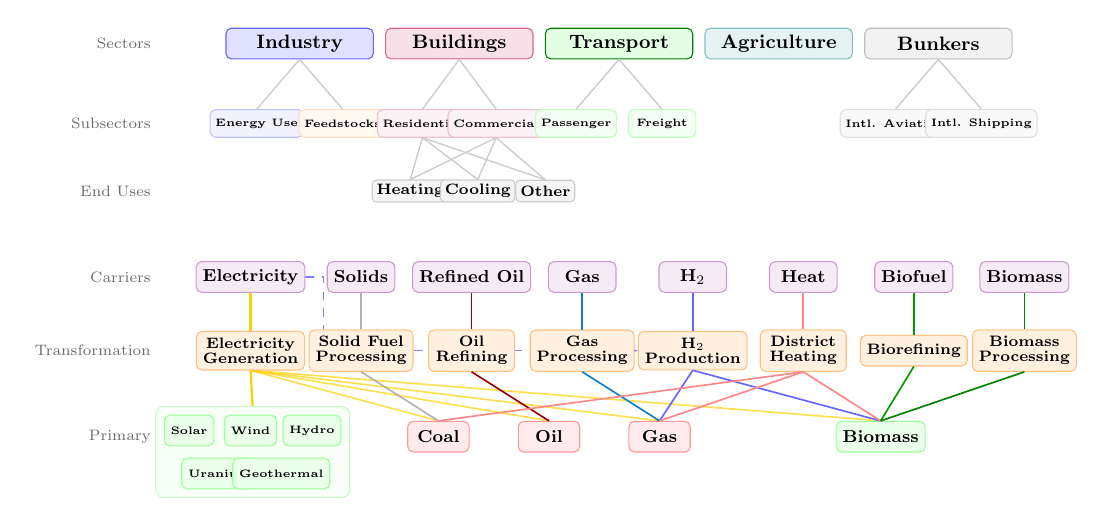
\begin{tikzpicture}[
  sbox/.style={rounded corners=2pt, minimum height=0.5cm, align=center,
               font=\footnotesize\bfseries, inner sep=3pt},
  ssbox/.style={rounded corners=2pt, minimum height=0.45cm, align=center,
               font=\scriptsize\bfseries, inner sep=2.5pt},
  tbox/.style={rounded corners=1.5pt, minimum height=0.35cm, align=center,
               font=\scriptsize\bfseries, inner sep=2pt, fill=gray!8, draw=gray!40},
  arr/.style={-{Stealth[length=3pt]}, gray!45, line width=0.6pt},
  arr2/.style={-{Stealth[length=2.5pt]}, gray!25, line width=0.4pt},
  byp/.style={-{Stealth[length=2.5pt]}, gray!30, dashed, line width=0.5pt},
  tree/.style={gray!40, line width=0.5pt},
  scale=0.78, transform shape,
]
  % ── Row 1: Sectors (y=0) ─────────────────────────────────────
  \node[sbox, fill=blue!12, draw=blue!60, minimum width=2.4cm, font=\small\bfseries] (ind) at (0.8,0) {Industry};
  \node[sbox, fill=purple!12, draw=purple!60, minimum width=2.4cm, font=\small\bfseries] (bld) at (3.4,0) {Buildings};
  \node[sbox, fill=green!10, draw=green!50!black, minimum width=2.4cm, font=\small\bfseries] (trn) at (6.0,0) {Transport};
  \node[sbox, fill=teal!10, draw=teal!50, minimum width=2.4cm, font=\small\bfseries] (agr) at (8.6,0) {Agriculture};
  \node[sbox, fill=gray!10, draw=gray!50, minimum width=2.4cm, font=\small\bfseries] (bnk) at (11.2,0) {Bunkers};

  % ── Row 2: Subsectors (y=-1.3) ──────────────────────────────
  % Industry
  \node[ssbox, fill=blue!5, draw=blue!25, minimum width=1.1cm, font=\tiny\bfseries] (euse) at (0.1,-1.3) {Energy Use};
  \node[ssbox, fill=orange!5, draw=orange!25, minimum width=1.1cm, font=\tiny\bfseries] (fs) at (1.5,-1.3) {Feedstocks};
  % Buildings
  \node[ssbox, fill=purple!5, draw=purple!25, minimum width=1.1cm, font=\tiny\bfseries] (res) at (2.8,-1.3) {Residential};
  \node[ssbox, fill=purple!5, draw=purple!25, minimum width=1.1cm, font=\tiny\bfseries] (com) at (4.0,-1.3) {Commercial};
  % Transport
  \node[ssbox, fill=green!5, draw=green!25, minimum width=1.1cm, font=\tiny\bfseries] (pas) at (5.3,-1.3) {Passenger};
  \node[ssbox, fill=green!5, draw=green!25, minimum width=1.1cm, font=\tiny\bfseries] (frt) at (6.7,-1.3) {Freight};
  % Agriculture: no subsectors
  % Bunkers
  \node[ssbox, fill=gray!5, draw=gray!25, minimum width=1.1cm, font=\tiny\bfseries] (bavia) at (10.5,-1.3) {Intl. Aviation};
  \node[ssbox, fill=gray!5, draw=gray!25, minimum width=1.1cm, font=\tiny\bfseries] (bship) at (11.9,-1.3) {Intl. Shipping};

  % ── Tree lines: Sector → Subsectors ─────────────────────────
  \foreach \s in {euse, fs} { \draw[tree] (ind.south) -- (\s.north); }
  \foreach \s in {res, com} { \draw[tree] (bld.south) -- (\s.north); }
  \foreach \s in {pas, frt} { \draw[tree] (trn.south) -- (\s.north); }
  \foreach \s in {bavia, bship} { \draw[tree] (bnk.south) -- (\s.north); }

  % ── Row 3: End Uses (y=-2.4) ─────────────────────────────────
  % Buildings end uses (shared by Residential & Commercial)
  \node[tbox] (eu_heat) at (2.6,-2.4) {Heating};
  \node[tbox] (eu_cool) at (3.7,-2.4) {Cooling};
  \node[tbox] (eu_oth)  at (4.8,-2.4) {Other};
  % Tree lines: both subsectors → same 3 end uses
  \foreach \s in {eu_heat, eu_cool, eu_oth} { \draw[tree] (res.south) -- (\s.north); }
  \foreach \s in {eu_heat, eu_cool, eu_oth} { \draw[tree] (com.south) -- (\s.north); }

  % ── Row 4: Carriers (y=-3.8) — aligned with transformation ──
  \def\cs{1.8}  % carrier/trans spacing
  \node[sbox, fill=violet!8, draw=violet!40, minimum width=1.1cm] (c_elec) at (0,-3.8)       {Electricity};
  \node[sbox, fill=violet!8, draw=violet!40, minimum width=1.1cm] (c_sol)  at (\cs*1,-3.8)   {Solids};
  \node[sbox, fill=violet!8, draw=violet!40, minimum width=1.2cm] (c_liq)  at (\cs*2,-3.8)   {Refined Oil};
  \node[sbox, fill=violet!8, draw=violet!40, minimum width=1.1cm] (c_gas)  at (\cs*3,-3.8)   {Gas};
  \node[sbox, fill=violet!8, draw=violet!40, minimum width=1.1cm] (c_h2)   at (\cs*4,-3.8)   {H$_2$};
  \node[sbox, fill=violet!8, draw=violet!40, minimum width=1.1cm] (c_heat) at (\cs*5,-3.8)   {Heat};
  \node[sbox, fill=violet!8, draw=violet!40, minimum width=1.1cm] (c_biof) at (\cs*6,-3.8)   {Biofuel};
  \node[sbox, fill=violet!8, draw=violet!40, minimum width=1.1cm] (c_bio)  at (\cs*7,-3.8)   {Biomass};

  % ── Row 5: Transformation (y=-5.0) — 8 items, uniform spacing ──
  \node[sbox, fill=orange!12, draw=orange!50, minimum width=1.4cm, font=\scriptsize\bfseries]
    (tr_elec) at (0,-5.0) {Electricity\\[-1pt]Generation};
  \node[sbox, fill=orange!12, draw=orange!50, minimum width=1.4cm, font=\scriptsize\bfseries]
    (tr_sfp)  at (\cs*1,-5.0) {Solid Fuel\\[-1pt]Processing};
  \node[sbox, fill=orange!12, draw=orange!50, minimum width=1.4cm, font=\scriptsize\bfseries]
    (tr_ref)  at (\cs*2,-5.0) {Oil\\[-1pt]Refining};
  \node[sbox, fill=orange!12, draw=orange!50, minimum width=1.4cm, font=\scriptsize\bfseries]
    (tr_gasp) at (\cs*3,-5.0) {Gas\\[-1pt]Processing};
  \node[sbox, fill=orange!12, draw=orange!50, minimum width=1.4cm, font=\scriptsize\bfseries]
    (tr_h2)   at (\cs*4,-5.0) {H$_2$\\[-1pt]Production};
  \node[sbox, fill=orange!12, draw=orange!50, minimum width=1.4cm, font=\scriptsize\bfseries]
    (tr_dh)   at (\cs*5,-5.0) {District\\[-1pt]Heating};
  \node[sbox, fill=orange!12, draw=orange!50, minimum width=1.4cm, font=\scriptsize\bfseries]
    (tr_bio)  at (\cs*6,-5.0) {Biorefining};
  \node[sbox, fill=orange!12, draw=orange!50, minimum width=1.4cm, font=\scriptsize\bfseries]
    (tr_bmp)  at (\cs*7,-5.0) {Biomass\\[-1pt]Processing};

  % ── Row 6: Primary (y=-6.4) ────────────────────────────────
  % Left group: elec-only (under Elec Gen)
  \node[sbox, fill=green!8, draw=green!40, minimum width=0.8cm, font=\tiny\bfseries] (p_sol)  at (-1.0,-6.3) {Solar};
  \node[sbox, fill=green!8, draw=green!40, minimum width=0.8cm, font=\tiny\bfseries] (p_wind) at (0,-6.3)    {Wind};
  \node[sbox, fill=green!8, draw=green!40, minimum width=0.8cm, font=\tiny\bfseries] (p_hyd)  at (1.0,-6.3)  {Hydro};
  \node[sbox, fill=green!8, draw=green!40, minimum width=0.8cm, font=\tiny\bfseries] (p_u)    at (-0.5,-7.0) {Uranium};
  \node[sbox, fill=green!8, draw=green!40, minimum width=1.0cm, font=\tiny\bfseries] (p_geo)  at (0.5,-7.0)  {Geothermal};
  \begin{pgfonlayer}{background}
    \node[rounded corners=3pt, draw=green!25, fill=green!3, line width=0.4pt,
          fit=(p_sol)(p_wind)(p_hyd)(p_u)(p_geo), inner sep=3pt] (epg) {};
  \end{pgfonlayer}
  % Right group: multi-use primaries
  \node[sbox, fill=red!8, draw=red!40, minimum width=1.0cm] (p_coal) at (\cs*1.7,-6.4) {Coal};
  \node[sbox, fill=red!8, draw=red!40, minimum width=1.0cm] (p_oil)  at (\cs*2.7,-6.4) {Oil};
  \node[sbox, fill=red!8, draw=red!40, minimum width=1.0cm] (p_gas)  at (\cs*3.7,-6.4) {Gas};
  \node[sbox, fill=green!8, draw=green!40, minimum width=1.0cm] (p_bio) at (\cs*5.7,-6.4) {Biomass};

  % ── Links ──────────────────────────────────────────────────
  % Elec-only primaries → Elec Gen → Electricity
  \draw[yellow!70!orange, line width=0.8pt] (epg.north) -- (tr_elec.south);
  \draw[yellow!70!orange, line width=0.8pt] (tr_elec.north) -- (c_elec.south);
  % Multi-use → Elec Gen (cross-link, faint)
  \begin{pgfonlayer}{background}
  \foreach \s in {p_coal, p_oil, p_gas, p_bio} {
    \draw[yellow!70!orange, line width=0.6pt, opacity=0.7] (\s.north) -- (tr_elec.south);
  }
  \end{pgfonlayer}
  % Solid Fuel Processing
  \draw[gray!60, line width=0.6pt] (p_coal.north) -- (tr_sfp.south);
  \draw[gray!60, line width=0.6pt] (tr_sfp.north) -- (c_sol.south);
  % Oil Refining
  \draw[red!60!black, line width=0.6pt] (p_oil.north) -- (tr_ref.south);
  \draw[red!60!black, line width=0.6pt] (tr_ref.north) -- (c_liq.south);
  % Gas Processing
  \draw[cyan!60!blue, line width=0.6pt] (p_gas.north) -- (tr_gasp.south);
  \draw[cyan!60!blue, line width=0.6pt] (tr_gasp.north) -- (c_gas.south);
  % H2 Production
  \draw[blue!60, line width=0.6pt] (p_gas.north) -- (tr_h2.south);
  \draw[blue!60, line width=0.6pt] (p_bio.north) -- (tr_h2.south);
  \draw[blue!60, line width=0.6pt] (tr_h2.north) -- (c_h2.south);
  % District Heating
  \foreach \s in {p_coal, p_gas, p_bio} {
    \draw[pink!70!red, line width=0.6pt] (\s.north) -- (tr_dh.south);
  }
  \draw[pink!70!red, line width=0.6pt] (tr_dh.north) -- (c_heat.south);
  % Biorefining
  \draw[green!60!black, line width=0.6pt] (p_bio.north) -- (tr_bio.south);
  \draw[green!60!black, line width=0.6pt] (tr_bio.north) -- (c_biof.south);
  % Biomass Processing
  \draw[green!50!black, line width=0.6pt] (p_bio.north) -- (tr_bmp.south);
  \draw[green!50!black, line width=0.6pt] (tr_bmp.north) -- (c_bio.south);
  % Electrolysis: Electricity → H2
  \begin{pgfonlayer}{background}
  \draw[-{Stealth[length=3pt]}, blue!50, line width=0.5pt, dashed]
    (c_elec.east) -- ++(0.3,0) |- (tr_h2.west);
  \end{pgfonlayer}

  % ── Row labels ───────────────────────────────────────────────
  \node[font=\scriptsize\color{TextLight}, anchor=east] at (-1.5,0) {Sectors};
  \node[font=\scriptsize\color{TextLight}, anchor=east] at (-1.5,-1.3) {Subsectors};
  \node[font=\scriptsize\color{TextLight}, anchor=east] at (-1.5,-2.4) {End Uses};
  \node[font=\scriptsize\color{TextLight}, anchor=east] at (-1.5,-3.8) {Carriers};
  \node[font=\scriptsize\color{TextLight}, anchor=east] at (-1.5,-5.0) {Transformation};
  \node[font=\scriptsize\color{TextLight}, anchor=east] at (-1.5,-6.4) {Primary};
\end{tikzpicture}
\end{frame}

% ── Slide: Industry ──────────────────────────────────────────────
\begin{frame}{Industry}
\centering
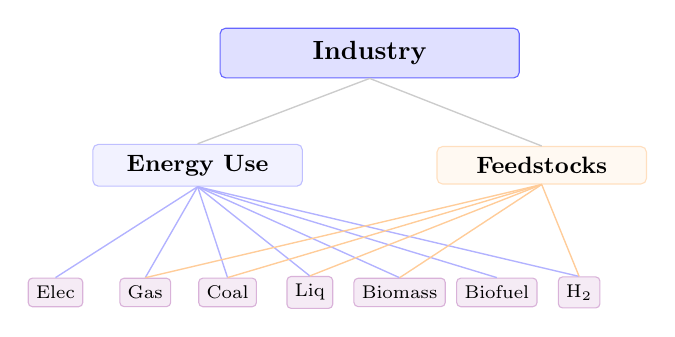
\begin{tikzpicture}[
  sbox/.style={rounded corners=2pt, minimum height=0.55cm, align=center,
               font=\normalsize\bfseries, inner sep=5pt},
  ssbox/.style={rounded corners=2pt, minimum height=0.5cm, align=center,
               font=\small\bfseries, inner sep=4pt},
  cbox/.style={font=\scriptsize, fill=violet!8, draw=violet!30, rounded corners=1.5pt, inner sep=3pt},
  fbox/.style={font=\scriptsize, fill=orange!8, draw=orange!30, rounded corners=1.5pt, inner sep=3pt},
  tree/.style={gray!40, line width=0.5pt},
  scale=0.95, transform shape,
]
  \node[sbox, fill=blue!12, draw=blue!60, minimum width=4cm] (ind) at (4.5,0) {Industry};

  \node[ssbox, fill=blue!5, draw=blue!25, minimum width=2.8cm] (eu) at (2.2,-1.5) {Energy Use};
  \node[ssbox, fill=orange!5, draw=orange!25, minimum width=2.8cm] (fs) at (6.8,-1.5) {Feedstocks};
  \foreach \s in {eu, fs} { \draw[tree] (ind.south) -- (\s.north); }

  % Shared carrier row
  \node[cbox] (c1) at (0.3,-3.2) {Elec};
  \node[cbox] (c2) at (1.5,-3.2) {Gas};
  \node[cbox] (c3) at (2.6,-3.2) {Coal};
  \node[cbox] (c4) at (3.7,-3.2) {Liq};
  \node[cbox] (c5) at (4.9,-3.2) {Biomass};
  \node[cbox] (c6) at (6.2,-3.2) {Biofuel};
  \node[cbox] (c7) at (7.3,-3.2) {H$_2$};

  % EU → carriers (blue lines)
  \foreach \s in {c1,c2,c3,c4,c5,c6,c7} { \draw[blue!30, line width=0.5pt] (eu.south) -- (\s.north); }
  % FS → carriers (orange lines)
  \foreach \s in {c2,c3,c4,c5,c7} { \draw[orange!40, line width=0.5pt] (fs.south) -- (\s.north); }
\end{tikzpicture}

\vspace{0.5em}
\raggedright
\small
$\bullet$~\textbf{Demand:} $\mathrm{Prod} = A_{\mathrm{prod}} \!\cdot\! \mathrm{Prod}_0 \!\cdot\! (Y/Y_0)^{\alpha} \!\cdot\! (P/P_0)^{\beta}$\\[3pt]
$\bullet$~\textbf{Energy Use:} $EU = ei_{EU} \!\cdot\! \mathrm{Prod}$\\[3pt]
$\bullet$~\textbf{Feedstocks:} $FS = ei_{FS} \!\cdot\! \mathrm{Prod}$\\[3pt]
$\bullet$~\textbf{Price Index:} $P = ei_{EU} \!\cdot\! P_{EU} + ei_{FS} \!\cdot\! P_{FS}$
\end{frame}

% ── Slide: Buildings ─────────────────────────────────────────────
\begin{frame}{Buildings}
\centering
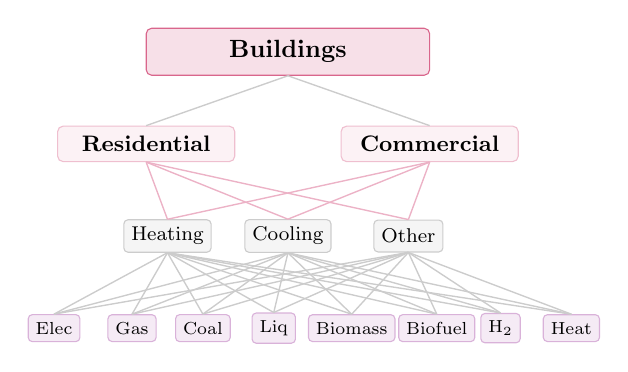
\begin{tikzpicture}[
  sbox/.style={rounded corners=2pt, minimum height=0.55cm, align=center,
               font=\normalsize\bfseries, inner sep=5pt},
  ssbox/.style={rounded corners=2pt, minimum height=0.5cm, align=center,
               font=\small\bfseries, inner sep=4pt},
  ebox/.style={rounded corners=1.5pt, minimum height=0.45cm, align=center,
               font=\footnotesize, inner sep=3pt, fill=gray!8, draw=gray!40},
  cbox/.style={font=\scriptsize, fill=violet!8, draw=violet!30, rounded corners=1.5pt, inner sep=3pt},
  tree/.style={gray!40, line width=0.5pt},
  scale=0.90, transform shape,
]
  \node[sbox, fill=purple!12, draw=purple!60, minimum width=4cm] (bld) at (4.5,0) {Buildings};

  \node[ssbox, fill=purple!5, draw=purple!25, minimum width=2.5cm] (res) at (2.5,-1.3) {Residential};
  \node[ssbox, fill=purple!5, draw=purple!25, minimum width=2.5cm] (com) at (6.5,-1.3) {Commercial};
  \foreach \s in {res, com} { \draw[tree] (bld.south) -- (\s.north); }

  % Shared end uses
  \node[ebox] (eu_h) at (2.8,-2.6) {Heating};
  \node[ebox] (eu_c) at (4.5,-2.6) {Cooling};
  \node[ebox] (eu_o) at (6.2,-2.6) {Other};
  \foreach \s in {eu_h, eu_c, eu_o} {
    \draw[purple!30, line width=0.5pt] (res.south) -- (\s.north);
    \draw[purple!30, line width=0.5pt] (com.south) -- (\s.north);
  }

  % Shared carriers (shifted right, Heat last)
  \node[cbox] (c1) at (1.2,-3.9) {Elec};
  \node[cbox] (c2) at (2.3,-3.9) {Gas};
  \node[cbox] (c3) at (3.3,-3.9) {Coal};
  \node[cbox] (c4) at (4.3,-3.9) {Liq};
  \node[cbox] (c5) at (5.4,-3.9) {Biomass};
  \node[cbox] (c6) at (6.6,-3.9) {Biofuel};
  \node[cbox] (c7) at (7.5,-3.9) {H$_2$};
  \node[cbox] (c8) at (8.5,-3.9) {Heat};
  \foreach \s in {c1,c2,c3,c4,c5,c6,c7,c8} {
    \draw[tree] (eu_h.south) -- (\s.north);
    \draw[tree] (eu_c.south) -- (\s.north);
    \draw[tree] (eu_o.south) -- (\s.north);
  }
\end{tikzpicture}

\end{frame}

% ── Slide: Buildings Demand 1/2 ──────────────────────────────────
\begin{frame}[t]{Buildings --- Demand (1/2): Floorspace}
\begin{columns}[T]
\column{0.52\textwidth}
\small
\vspace{0.2em}

\textbf{Step 1: Per-capita floorspace}\\[2pt]
{\scriptsize Saturates with income --- rich countries plateau.}
\vspace{-0.3em}
$$FS_{pc} = (\bar{F}\!-\!F_{\min})\!\left(1 - e^{\frac{-\ln 2}{\tilde{y}}\, y_{pc}\, (P/P_0)^{\beta}}\right) + F_{\min}$$
\vspace{-1.0em}
\begin{itemize}\setlength\itemsep{2pt}\setlength\parsep{0pt}
\item[\scriptsize$\bullet$] {\scriptsize $\bar{F}$: satiation level (m$^2$/cap)}
\item[\scriptsize$\bullet$] {\scriptsize $\tilde{y}$: midpoint income (50\% of $\bar{F}$)}
\item[\scriptsize$\bullet$] {\scriptsize $F_{\min}$: subsistence floor}
\item[\scriptsize$\bullet$] {\scriptsize $P/P_0$: housing price index (relative to base year)}
\item[\scriptsize$\bullet$] {\scriptsize $\beta$: price elasticity of floorspace}
\item[\scriptsize$\bullet$] {\scriptsize Floor: $FS_{pc} \geq FS_{pc,\mathrm{base}}$ (no shrinkage)}
\end{itemize}

\vspace{0.4em}
\textbf{Step 2: Total floorspace}
\vspace{-0.3em}
$$FS(t) = FS_{pc}(t) \times \mathrm{Pop}(t)$$

\column{0.46\textwidth}
\centering
\vspace{0.2em}
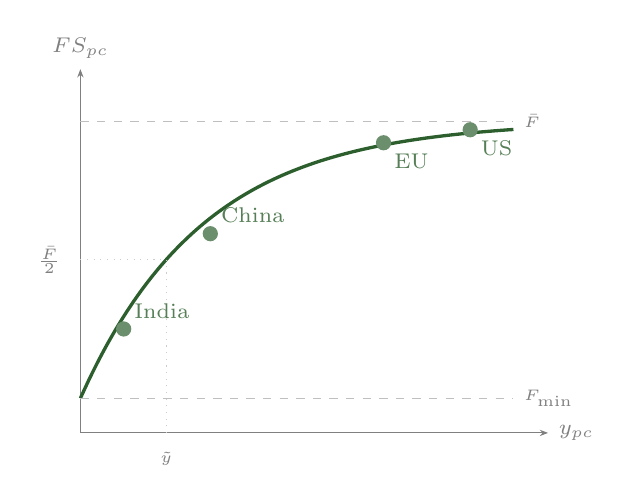
\begin{tikzpicture}[scale=1.1, transform shape]
  \draw[-{Stealth[length=3pt]}, gray] (0,0) -- (5.4,0) node[right, font=\scriptsize] {$y_{pc}$};
  \draw[-{Stealth[length=3pt]}, gray] (0,0) -- (0,4.2) node[above, font=\scriptsize] {$FS_{pc}$};
  % Satiation curve
  \draw[SpruceGreen, line width=1.2pt, smooth, domain=0:5, samples=50]
    plot (\x, {0.4 + 3.2*(1 - exp(-0.7*\x))});
  % Satiation line
  \draw[dashed, gray!50] (0,3.6) -- (5,3.6) node[right, font=\tiny, text=gray] {$\bar{F}$};
  % F_min line
  \draw[dashed, gray!50] (0,0.4) -- (5,0.4) node[right, font=\tiny, text=gray] {$F_{\min}$};
  % Midpoint
  \draw[dotted, gray!40] (0.99,0) -- (0.99,2.0);
  \draw[dotted, gray!40] (0,2.0) -- (0.99,2.0);
  \node[font=\tiny, text=gray] at (0.99,-0.3) {$\tilde{y}$};
  \node[font=\tiny, text=gray, anchor=east] at (-0.1,2.0) {$\frac{\bar{F}}{2}$};
  % Region labels
  \fill[SpruceGreen!70] (0.5,1.2) circle (2.5pt) node[above right, font=\scriptsize, text=SpruceGreen!80] {India};
  \fill[SpruceGreen!70] (1.5,2.3) circle (2.5pt) node[above right, font=\scriptsize, text=SpruceGreen!80] {China};
  \fill[SpruceGreen!70] (3.5,3.35) circle (2.5pt) node[below right, font=\scriptsize, text=SpruceGreen!80] {EU};
  \fill[SpruceGreen!70] (4.5,3.5) circle (2.5pt) node[below right, font=\scriptsize, text=SpruceGreen!80] {US};
\end{tikzpicture}
\end{columns}
\end{frame}

% ── Slide: Buildings Demand 2/2 ──────────────────────────────────
\begin{frame}[t]{Buildings --- Demand (2/2): Service Intensity \& Energy}
\begin{columns}[T]
\column{0.52\textwidth}
\small
\vspace{0.1em}

\textbf{Step 3: Service intensity per m$^2$}\\[1pt]
{\scriptsize Thermal load $\times$ service density per unit floor.}
\vspace{-0.4em}
$$I_{svc}(t) = \underbrace{DD(t) \cdot U(t)}_{\text{thermal load}} \times \underbrace{d_{svc}\!\left(\frac{y_{pc}}{P_{svc}}\right)}_{\text{service density}}$$
\vspace{-1.2em}
\begin{itemize}\setlength\itemsep{1pt}\setlength\parsep{0pt}
\item[\scriptsize$\bullet$] {\scriptsize $DD$: degree days (HDD for heating, CDD for cooling)}
\item[\scriptsize$\bullet$] {\scriptsize $U(t)$: shell conductance --- improves over time}
\item[\scriptsize$\bullet$] {\scriptsize $d_{svc}$: satiation function of \textit{affordability} ($y_{pc}/P_{svc}$)}
\item[\scriptsize$\bullet$] {\scriptsize Non-thermal (lighting, etc.): no $DD$ term}
\end{itemize}

\vspace{0.2em}
\textbf{Step 4: Energy demand by service}
\vspace{-0.4em}
$$E_{svc}(t) = FS(t) \cdot I_{svc}(t) \cdot \sum_c \frac{s_c}{eff_c^{svc}}$$
\vspace{-1.2em}
\begin{itemize}\setlength\itemsep{1pt}\setlength\parsep{0pt}
\item[\scriptsize$\bullet$] {\scriptsize $s_c$: carrier share from logit}
\item[\scriptsize$\bullet$] {\scriptsize $eff_c^{svc}$: service efficiency of carrier $c$}
\end{itemize}

\column{0.46\textwidth}
\centering
\vspace{0.2em}
{\footnotesize\bfseries Service density $d_{svc}$}\\[3pt]
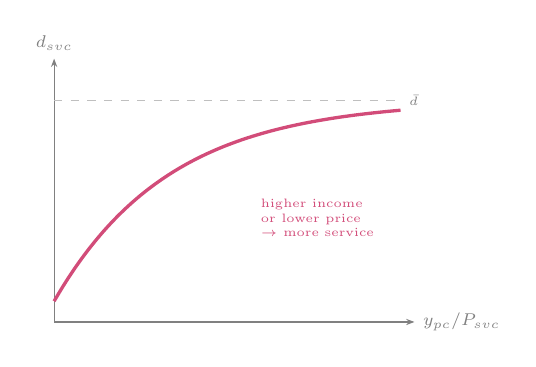
\begin{tikzpicture}[scale=0.88, transform shape]
  \draw[-{Stealth[length=3pt]}, gray] (0,0) -- (5.2,0) node[right, font=\scriptsize] {$y_{pc}/P_{svc}$};
  \draw[-{Stealth[length=3pt]}, gray] (0,0) -- (0,3.8) node[above, font=\scriptsize] {$d_{svc}$};
  % Satiation curve
  \draw[purple!70, line width=1.2pt, smooth, domain=0:5, samples=50]
    plot (\x, {0.3 + 2.9*(1 - exp(-0.6*\x))});
  % Satiation line
  \draw[dashed, gray!50] (0,3.2) -- (5,3.2) node[right, font=\tiny, text=gray] {$\bar{d}$};
  % Annotations
  \node[font=\tiny, text=purple!70, align=left] at (3.8,1.5) {higher income\\or lower price\\$\to$ more service};
\end{tikzpicture}

\vspace{0.2em}
{\footnotesize\bfseries Service price}\\[2pt]
\begin{tcolorbox}[enhanced, colback=gray!4, colframe=gray!40, boxrule=0.4pt, arc=2pt,
  left=3pt, right=3pt, top=2pt, bottom=2pt]
\scriptsize
$P_{svc} = \sum_c s_c \cdot C_c / eff_c^{svc}$ \;{\tiny(cost/GJ-service)}\\[2pt]
{\tiny\textbullet\; Gas: $eff^{svc}_{gas} \approx 0.9$}\\
{\tiny\textbullet\; Elec: $eff^{svc}_{elec} \approx 3.0$ (heat pump)}
\end{tcolorbox}
\end{columns}
\end{frame}

% ── Slide: Transport ─────────────────────────────────────────────
\begin{frame}{Transport}
\centering
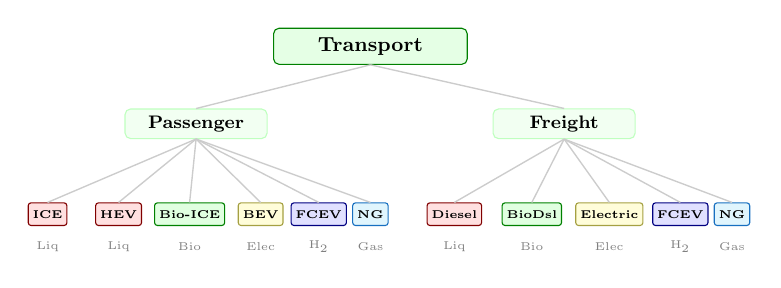
\begin{tikzpicture}[
  sbox/.style={rounded corners=2pt, minimum height=0.5cm, align=center,
               font=\small\bfseries, inner sep=4pt},
  ssbox/.style={rounded corners=2pt, minimum height=0.45cm, align=center,
               font=\footnotesize\bfseries, inner sep=3pt},
  pt/.style={rounded corners=1pt, minimum height=0.35cm, align=center,
             font=\tiny\bfseries, inner sep=2pt},
  tree/.style={gray!40, line width=0.5pt},
  scale=0.82, transform shape,
]
  % Transport root
  \node[sbox, fill=green!10, draw=green!50!black, minimum width=3cm] (trn) at (5.5,0) {Transport};

  % Subsectors
  \node[ssbox, fill=green!5, draw=green!25, minimum width=2.2cm] (pas) at (2.8,-1.2) {Passenger};
  \node[ssbox, fill=green!5, draw=green!25, minimum width=2.2cm] (frt) at (8.5,-1.2) {Freight};
  \draw[tree] (trn.south) -- (pas.north);
  \draw[tree] (trn.south) -- (frt.north);

  % ── Passenger powertrains (6) — colored by fuel carrier ──
  \node[pt, fill=red!12, draw=red!50!black] (p1) at (0.5,-2.6) {ICE};
  \node[pt, fill=red!12, draw=red!50!black] (p2) at (1.6,-2.6) {HEV};
  \node[pt, fill=green!12, draw=green!50!black] (p3) at (2.7,-2.6) {Bio-ICE};
  \node[pt, fill=yellow!15, draw=yellow!60!black] (p4) at (3.8,-2.6) {BEV};
  \node[pt, fill=blue!12, draw=blue!50!black] (p5) at (4.7,-2.6) {FCEV};
  \node[pt, fill=cyan!12, draw=cyan!50!blue] (p6) at (5.5,-2.6) {NG};
  \foreach \s in {p1,p2,p3,p4,p5,p6} { \draw[tree] (pas.south) -- (\s.north); }

  % Fuel labels under passenger powertrains
  \node[font=\tiny, text=gray] at (0.5,-3.1) {Liq};
  \node[font=\tiny, text=gray] at (1.6,-3.1) {Liq};
  \node[font=\tiny, text=gray] at (2.7,-3.1) {Bio};
  \node[font=\tiny, text=gray] at (3.8,-3.1) {Elec};
  \node[font=\tiny, text=gray] at (4.7,-3.1) {H$_2$};
  \node[font=\tiny, text=gray] at (5.5,-3.1) {Gas};

  % ── Freight powertrains (5) — colored by fuel carrier ──
  \node[pt, fill=red!12, draw=red!50!black] (f1) at (6.8,-2.6) {Diesel};
  \node[pt, fill=green!12, draw=green!50!black] (f2) at (8.0,-2.6) {BioDsl};
  \node[pt, fill=yellow!15, draw=yellow!60!black] (f3) at (9.2,-2.6) {Electric};
  \node[pt, fill=blue!12, draw=blue!50!black] (f4) at (10.3,-2.6) {FCEV};
  \node[pt, fill=cyan!12, draw=cyan!50!blue] (f5) at (11.1,-2.6) {NG};
  \foreach \s in {f1,f2,f3,f4,f5} { \draw[tree] (frt.south) -- (\s.north); }

  % Fuel labels under freight powertrains
  \node[font=\tiny, text=gray] at (6.8,-3.1) {Liq};
  \node[font=\tiny, text=gray] at (8.0,-3.1) {Bio};
  \node[font=\tiny, text=gray] at (9.2,-3.1) {Elec};
  \node[font=\tiny, text=gray] at (10.3,-3.1) {H$_2$};
  \node[font=\tiny, text=gray] at (11.1,-3.1) {Gas};

\end{tikzpicture}

\vspace{0.3em}
\small
\begin{itemize}\setlength\itemsep{3pt}\setlength\parsep{0pt}
\item Demand: $SD = sd_{pc,0} \!\cdot\! \left(\frac{GDP_{pc}}{GDP_{pc,0}}\right)^{\!\alpha} \!\cdot\! \left(\frac{P}{P_0}\right)^{\!\beta} \times \mathrm{Pop}$
\item Energy: $E = \sum_i SD \cdot s_i / eff_i$
\item LCOT: $\dfrac{capex \cdot FCR}{annual\text{-}SD} + \dfrac{C_{fuel}}{eff} + O\!\&\!M + \dfrac{VOT}{speed}$
\begin{itemize}\setlength\itemsep{1pt}\setlength\parsep{0pt}
\item[\scriptsize$\bullet$] {\scriptsize $FCR$: annualized capital recovery rate}
\item[\scriptsize$\bullet$] {\scriptsize $VOT$: value of time ($GDP_{pc}$/hrs\_yr, \$/hr)}
\end{itemize}
\end{itemize}
\end{frame}

% ── Slide: Agriculture ──────────────────────────────────────────
\begin{frame}{Agriculture}
\centering
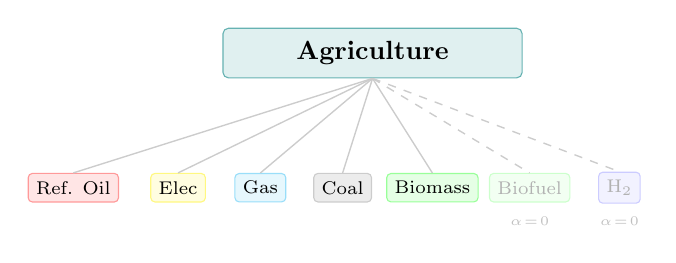
\begin{tikzpicture}[
  sbox/.style={rounded corners=2pt, minimum height=0.55cm, align=center,
               font=\normalsize\bfseries, inner sep=5pt},
  cbox/.style={font=\scriptsize, rounded corners=1.5pt, inner sep=3pt},
  tree/.style={gray!40, line width=0.5pt},
  scale=0.95, transform shape,
]
  % Root node
  \node[sbox, fill=teal!12, draw=teal!60, minimum width=4cm] (ag) at (4.5,0) {Agriculture};

  % Carrier row — 7 carriers
  \node[cbox, fill=red!10,    draw=red!40]    (c1) at (0.5,-1.8) {Ref. Oil};
  \node[cbox, fill=yellow!12, draw=yellow!50] (c2) at (1.9,-1.8) {Elec};
  \node[cbox, fill=cyan!10,   draw=cyan!40]   (c3) at (3.0,-1.8) {Gas};
  \node[cbox, fill=gray!15,   draw=gray!40]   (c4) at (4.1,-1.8) {Coal};
  \node[cbox, fill=green!10,  draw=green!40]  (c5) at (5.3,-1.8) {Biomass};
  \node[cbox, fill=green!5,   draw=green!20, text=gray!60]  (c6) at (6.6,-1.8) {Biofuel};
  \node[cbox, fill=blue!5,    draw=blue!20, text=gray!60]   (c7) at (7.8,-1.8) {H$_2$};

  \foreach \s in {c1,c2,c3,c4,c5} { \draw[tree] (ag.south) -- (\s.north); }
  \foreach \s in {c6,c7} { \draw[tree, dashed] (ag.south) -- (\s.north); }

  % α=0 labels
  \node[font=\tiny, text=gray!50] at (6.6,-2.25) {$\alpha\!=\!0$};
  \node[font=\tiny, text=gray!50] at (7.8,-2.25) {$\alpha\!=\!0$};
\end{tikzpicture}

\vspace{0.4em}
\raggedright
\small
\begin{itemize}\setlength\itemsep{3pt}\setlength\parsep{0pt}
\item \textbf{Ag.\ Output:} $Q_{ag} = Q_0 \!\cdot\! \left(\frac{GDP}{GDP_0}\right)^{\!\alpha_{ag}} \!\cdot\! \left(\frac{P_{ag}}{P_0}\right)^{\!\gamma_{ag}}$
\item \textbf{Energy:} $E_{ag} = ei_{ag} \times Q_{ag}$
\end{itemize}
\end{frame}

% ── Slide: Bunkers ──────────────────────────────────────────────
\begin{frame}{Bunkers (International Aviation \& Shipping)}
\centering
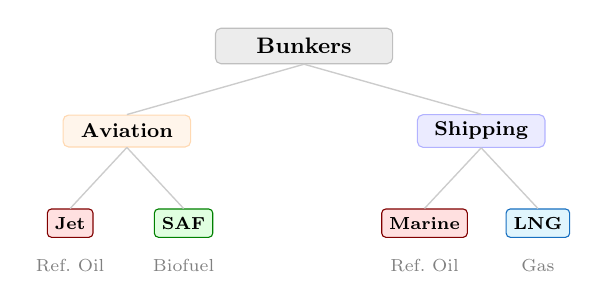
\begin{tikzpicture}[
  sbox/.style={rounded corners=2pt, minimum height=0.5cm, align=center,
               font=\small\bfseries, inner sep=4pt},
  ssbox/.style={rounded corners=2pt, minimum height=0.45cm, align=center,
               font=\footnotesize\bfseries, inner sep=3pt},
  pt/.style={rounded corners=1.5pt, minimum height=0.4cm, align=center,
             font=\scriptsize\bfseries, inner sep=3pt},
  tree/.style={gray!40, line width=0.5pt},
  scale=0.90, transform shape,
]
  % Root node
  \node[sbox, fill=gray!15, draw=gray!50, minimum width=2.5cm] (bkr) at (5.5,0) {Bunkers};

  % Subsectors
  \node[ssbox, fill=orange!8, draw=orange!30, minimum width=1.8cm] (avi) at (3.0,-1.2) {Aviation};
  \node[ssbox, fill=blue!8, draw=blue!30, minimum width=1.8cm]     (shp) at (8.0,-1.2) {Shipping};
  \draw[tree] (bkr.south) -- (avi.north);
  \draw[tree] (bkr.south) -- (shp.north);

  % Aviation powertrains
  \node[pt, fill=red!12,   draw=red!50!black]   (a1) at (2.2,-2.5) {Jet};
  \node[pt, fill=green!12, draw=green!50!black]  (a2) at (3.8,-2.5) {SAF};
  \foreach \s in {a1,a2} { \draw[tree] (avi.south) -- (\s.north); }

  % Fuel labels under aviation
  \node[font=\scriptsize, text=gray] at (2.2,-3.1) {Ref.\ Oil};
  \node[font=\scriptsize, text=gray] at (3.8,-3.1) {Biofuel};

  % Shipping powertrains
  \node[pt, fill=red!12,  draw=red!50!black]  (s1) at (7.2,-2.5) {Marine};
  \node[pt, fill=cyan!12, draw=cyan!50!blue]  (s2) at (8.8,-2.5) {LNG};
  \foreach \s in {s1,s2} { \draw[tree] (shp.south) -- (\s.north); }

  % Fuel labels under shipping
  \node[font=\scriptsize, text=gray] at (7.2,-3.1) {Ref.\ Oil};
  \node[font=\scriptsize, text=gray] at (8.8,-3.1) {Gas};

\end{tikzpicture}

\vspace{0.3em}
\raggedright
\small
\begin{itemize}\setlength\itemsep{3pt}\setlength\parsep{0pt}
\item \textbf{Aviation:} $E_{avi} = E_0 \!\cdot\! (GDP_{world}/GDP_0)^{\alpha_{avi}}$
\item \textbf{Shipping:} $E_{ship} = E_0 \!\cdot\! (GDP_{world}/GDP_0)^{\alpha_{ship}}$
\item \textbf{LCOT:} $\dfrac{capex \!\cdot\! FCR}{annual\text{-}SD} + \dfrac{C_{fuel}}{eff} + O\!\&\!M$
\end{itemize}
\end{frame}

% ── Slide: Energy Supply Chain ──────────────────────────────────
\begin{frame}{Energy Supply Chain}
\centering
\pgfdeclarelayer{background}
\pgfsetlayers{background,main}
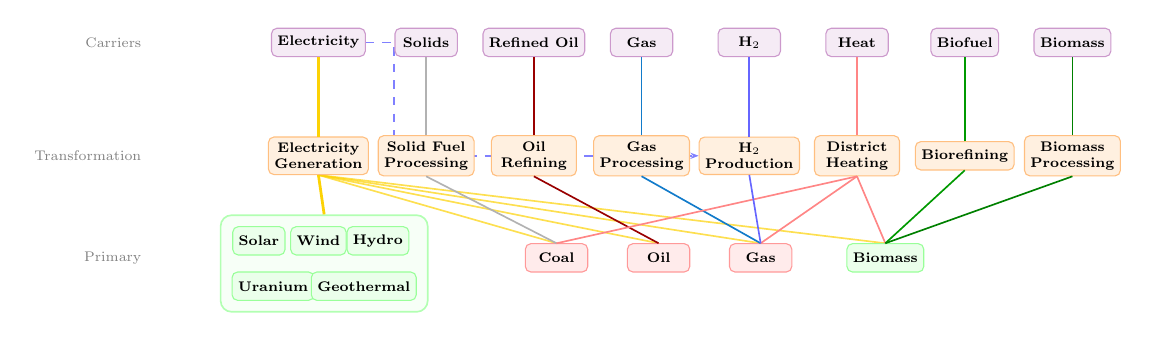
\begin{tikzpicture}[
  sbox/.style={rounded corners=2pt, minimum height=0.5cm, align=center,
               font=\scriptsize\bfseries, inner sep=3pt},
  tbox/.style={rounded corners=2pt, minimum height=0.5cm, align=center,
               font=\scriptsize\bfseries, inner sep=3pt,
               fill=orange!12, draw=orange!50},
  pbox/.style={rounded corners=2pt, minimum height=0.5cm, align=center,
               font=\scriptsize\bfseries, inner sep=3pt},
  cbox/.style={rounded corners=2pt, minimum height=0.5cm, align=center,
               font=\scriptsize\bfseries, inner sep=3pt,
               fill=violet!8, draw=violet!40},
  link/.style={line width=0.6pt},
  bypass/.style={line width=0.6pt, dashed},
  scale=0.72, transform shape,
]
  % Layout: Left = Elec-only column, Right = Multi-use grid
  % Rows: Carriers (y=0), Transformation (y=-2), Primary (y=-3.8)

  % ═══ LEFT: Electricity-only column ═══════════════════════════
  % Carrier
  \node[cbox, minimum width=1.6cm] (c_elec) at (0, 0) {Electricity};

  % Transformation
  \node[tbox, minimum width=1.5cm] (tr_elec) at (0, -2) {Electricity\\Generation};

  % Primaries (elec-only) — grouped box
  \node[pbox, fill=green!8, draw=green!40, minimum width=0.9cm] (p_sol)  at (-1.05, -3.5) {Solar};
  \node[pbox, fill=green!8, draw=green!40, minimum width=0.9cm] (p_wind) at (0, -3.5)     {Wind};
  \node[pbox, fill=green!8, draw=green!40, minimum width=0.9cm] (p_hyd)  at (1.05, -3.5)  {Hydro};
  \node[pbox, fill=green!8, draw=green!40, minimum width=1.0cm] (p_u)    at (-0.8, -4.3)  {Uranium};
  \node[pbox, fill=green!8, draw=green!40, minimum width=1.2cm] (p_geo)  at (0.8, -4.3)   {Geothermal};
  % Group outline
  \begin{pgfonlayer}{background}
    \node[rounded corners=4pt, draw=green!30, fill=green!3, line width=0.6pt,
          fit=(p_sol)(p_wind)(p_hyd)(p_u)(p_geo), inner sep=4pt] (elec_prim_group) {};
  \end{pgfonlayer}

  % Links: Group → Elec Gen → Electricity
  \draw[yellow!70!orange, link, line width=1pt] (elec_prim_group.north) -- (tr_elec.south);
  \draw[yellow!70!orange, link, line width=1pt] (tr_elec.north) -- (c_elec.south);

  % (no separator line)

  % ═══ RIGHT: Multi-use primaries ═════════════════════════════
  % Carriers (right side) — center-aligned with corresponding transformation
  \node[cbox, minimum width=1.1cm] (c_sol)  at (1.9, 0)  {Solids};
  \node[cbox, minimum width=1.3cm] (c_liq)  at (3.8, 0)  {Refined Oil};
  \node[cbox, minimum width=1.1cm] (c_gas)  at (5.7, 0)  {Gas};
  \node[cbox, minimum width=1.1cm] (c_h2)   at (7.6, 0)  {H$_2$};
  \node[cbox, minimum width=1.1cm] (c_heat) at (9.5, 0)  {Heat};
  \node[cbox, minimum width=1.1cm] (c_biof) at (11.4, 0) {Biofuel};
  \node[cbox, minimum width=1.1cm] (c_bio)  at (13.3, 0) {Biomass};

  % Transformation (right side): SFP, OR, GP, H₂, DH, Biorefining, BP
  \node[tbox, minimum width=1.5cm] (tr_sfp)  at (1.9, -2)  {Solid Fuel\\Processing};
  \node[tbox, minimum width=1.5cm] (tr_ref)  at (3.8, -2)  {Oil\\Refining};
  \node[tbox, minimum width=1.5cm] (tr_gasp) at (5.7, -2)  {Gas\\Processing};
  \node[tbox, minimum width=1.5cm] (tr_h2)   at (7.6, -2)  {H$_2$\\Production};
  \node[tbox, minimum width=1.5cm] (tr_dh)   at (9.5, -2)  {District\\Heating};
  \node[tbox, minimum width=1.5cm] (tr_bio)  at (11.4, -2) {Biorefining};
  \node[tbox, minimum width=1.5cm] (tr_bmp)  at (13.3, -2) {Biomass\\Processing};

  % Primaries (multi-use) — fossil + biomass
  \node[pbox, fill=red!8, draw=red!40, minimum width=1.1cm] (p_coal) at (4.2, -3.8)  {Coal};
  \node[pbox, fill=red!8, draw=red!40, minimum width=1.1cm] (p_oil)  at (6.0, -3.8)  {Oil};
  \node[pbox, fill=red!8, draw=red!40, minimum width=1.1cm] (p_gas)  at (7.8, -3.8)  {Gas};
  \node[pbox, fill=green!8, draw=green!40, minimum width=1.1cm] (p_bio) at (10.0, -3.8) {Biomass};

  % ═══ Links: Multi-use ═══════════════════════════════════════
  % Gas Processing
  \draw[cyan!60!blue, link] (p_gas.north) -- (tr_gasp.south);
  \draw[cyan!60!blue, link] (tr_gasp.north) -- (c_gas.south);
  % Oil Refining
  \draw[red!60!black, link] (p_oil.north) -- (tr_ref.south);
  \draw[red!60!black, link] (tr_ref.north) -- (c_liq.south);
  % Solid Fuel Processing
  \draw[gray!60, link] (p_coal.north) -- (tr_sfp.south);
  \draw[gray!60, link] (tr_sfp.north) -- (c_sol.south);
  % District Heating (coal, oil, gas, biomass → heat)
  \foreach \s in {p_coal, p_gas, p_bio} {
    \draw[pink!70!red, link] (\s.north) -- (tr_dh.south);
  }
  \draw[pink!70!red, link] (tr_dh.north) -- (c_heat.south);
  % H2 Production (gas, biomass → H2)
  \draw[blue!60, link] (p_gas.north) -- (tr_h2.south);
  \draw[blue!60, link] (tr_h2.north) -- (c_h2.south);
  % Biorefining (biomass → biofuel)
  \draw[green!60!black, link] (p_bio.north) -- (tr_bio.south);
  \draw[green!60!black, link] (tr_bio.north) -- (c_biof.south);
  % Biomass Processing (biomass → biomass carrier)
  \draw[green!50!black, link] (p_bio.north) -- (tr_bmp.south);
  \draw[green!50!black, link] (tr_bmp.north) -- (c_bio.south);

  % Multi-use primaries also feed Elec Gen (cross-link)
  \begin{pgfonlayer}{background}
  \foreach \s in {p_coal, p_oil, p_gas, p_bio} {
    \draw[yellow!70!orange, link, opacity=0.7] (\s.north) -- (tr_elec.south);
  }
  % Electrolysis: Electricity → H2 Production
  \draw[-{Stealth[length=3pt]}, blue!50, bypass] (c_elec.east)
    -- ++(0.5,0) |- (tr_h2.west);
  \end{pgfonlayer}

  % ═══ Row labels ═════════════════════════════════════════════
  \node[font=\scriptsize\color{gray}, anchor=east] at (-3.0, 0)    {Carriers};
  \node[font=\scriptsize\color{gray}, anchor=east] at (-3.0, -2)   {Transformation};
  \node[font=\scriptsize\color{gray}, anchor=east] at (-3.0, -3.8) {Primary};
\end{tikzpicture}
\end{frame}

% ── Slide: Primary Energy Supply — Fossil Fuels ─────────────────
\begin{frame}{Primary Energy Supply --- Fossil Fuels}
\small
\textbf{Grade-based supply curves} for coal, oil, gas per region --- higher prices unlock higher-cost grades.

\vspace{0.3em}
\centering
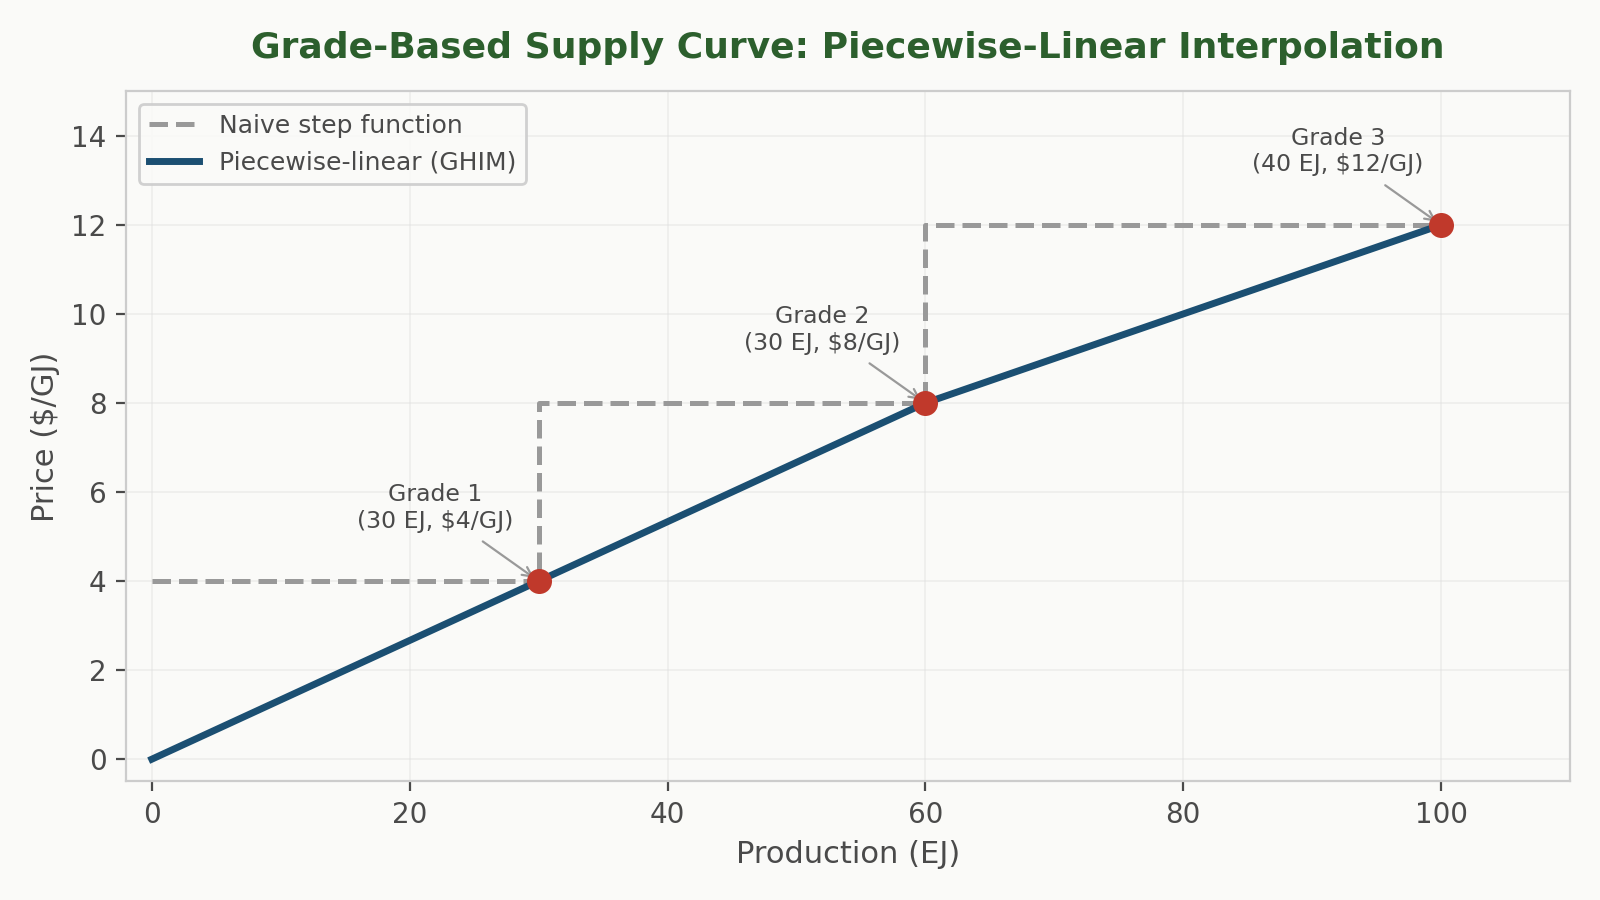
\includegraphics[width=0.78\linewidth]{supply_curve.png}
\end{frame}

% (Merged into Two-Factor Learning slide below)


% ── Slide 14: Inter-Regional Trade ───────────────────────────────
\begin{frame}[t]{Inter-Regional Trade --- Global Market Clearing}
\vspace{0.3em}
\textbf{\underline{Global Market Clearing}}
\bi \small
  \item Single world price $p^*$ per fuel (coal, oil, gas)
  \item $\sum_r Q^s_r(p^*) = \sum_r Q^d_r(p^*)$ \quad (supply = demand)
  \item Net trade: $X_r = Q^s_r - Q^d_r$
\ei

\vspace{0.8em}
\textbf{\underline{Calibration Rent}} {\small (region-specific, fixed at base year)}
\bi \small
  \item $\mathrm{rent}_r = P_{\mathrm{observed}} - P_{\mathrm{cleared}}$ \quad per region $r$
  \item Carried forward as price adder into all future clearing
  \item Supply evaluated at extraction cost $+$ $\mathrm{rent}_r$
\ei
\end{frame}

\section{Technology Choice}


% ── Slide 15: Technology Share ────────────────────────────────────
\begin{frame}[t]{Technology Share}

\begin{tcolorbox}[enhanced, colback=green!4, colframe=green!30, boxrule=0.5pt, arc=2pt]
\centering
$s_i = \dfrac{\alpha_i \cdot e^{\,\beta \, C_i + p_i}}{\sum_j \alpha_j \cdot e^{\,\beta \, C_j + p_j}}$
\end{tcolorbox}

\vspace{0.2em}
\begin{tcolorbox}[goalbox, colback=green!6, colframe=green!50!black, top=2pt, bottom=2pt, title={\color{white}\small $\alpha_i$ \; Availability Switch}]
\scriptsize Gate $\{0,1\}$: ban / enable technologies via policy
\end{tcolorbox}
\vspace{-0.15em}
\begin{tcolorbox}[goalbox, colback=orange!6, colframe=orange!70!black, top=2pt, bottom=2pt, title={\color{white}\small $p_i$ \; Preference Weight}]
\scriptsize SSP-calibrated non-cost factor; decays over time
\end{tcolorbox}
\vspace{-0.15em}
\begin{tcolorbox}[goalbox, colback=blue!6, colframe=blue!60, top=2pt, bottom=2pt, title={\color{white}\small $C_i$ \; Cost (\$/GJ)}]
\scriptsize
\bi
  \item LCOE: capex + O\&M + fuel
  \item LCOT: LCOE + time value
\ei
\end{tcolorbox}

\end{frame}

% ── Slide: Two-Factor Learning (RND + LBD) ──────────────────────
\begin{frame}[t]{Two-Factor Learning}
\small
Capital cost declines with cumulative deployment and R\&D:

\vspace{0.3em}
\centering
\large
$\mathrm{capex}_j(t) = \mathrm{capex}_{j,0} \times \underbrace{\Bigl(\dfrac{Q_j^{\mathrm{cum}}}{Q_{j,0}}\Bigr)^{-\alpha}}_{\text{LBD}} \times \underbrace{\Bigl(\dfrac{H_j^{\mathrm{RD}}}{H_{j,0}}\Bigr)^{-\beta}}_{\text{RND}}$
\hspace{1.5em}
\small Floor: $0.2 \times \mathrm{capex}_0$

\vspace{0.5em}
\flushleft
\small
\textbullet\ \textbf{LBD} (Learning by Doing): cost $\downarrow$ with cumulative deployment $Q_j^{\mathrm{cum}}$\\
\textbullet\ \textbf{RND} (Research \& Development): cost $\downarrow$ with RND knowledge stock $H_j^{\mathrm{RD}}$

\vspace{0.4em}
\centering
\scriptsize
\begin{tabular}{l c c}
\toprule
\textbf{Technology} & \textbf{LBD Rate} & \textbf{RND Channel} \\
\midrule
Solar        & 20\% & High \\
Wind         & 12\% & Medium \\
Nuclear      & 3\%  & Low \\
Electrolysis & 15\% & High \\
Batteries (EV)  & 10\% & High \\
Heat pumps      & 10\% & Medium \\
CCS             & 5\%  & Medium \\
H$_2$ DRI       & 8\%  & Medium \\
\bottomrule
\end{tabular}
\end{frame}

% ── Slide 16: Vintage Retirement — Combined Framework ────────────
\begin{frame}[t]{Vintage Retirement}
\small Capacity at vintage $v$ survives only if the plant is both young enough \textbf{AND} profitable enough.

\vspace{0.2em}
\centering
$Q_{\mathrm{eff}}(t) = \sum_v C_{i,v}\cdot S_i(t-v)\cdot P(\pi_{i,v})$

\vspace{0.4em}
\begin{tcolorbox}[infobox, colback=blue!6, colframe=blue!60, top=2pt, bottom=2pt, title=Age-Based Survival \; $S(\mathrm{age})$]
\small
$S(a) = \dfrac{1/(1+e^{k(a-\rho L)})}{S(0)}$

\smallskip
\scriptsize
\bi
  \item $\rho=0.75$ (half-life ratio), $k=0.1$ (steepness)
  \item Lifetime $L$ differs by technology
  \item Renewables: hard cutoff at $L$ (no S-curve)
\ei
\end{tcolorbox}
\vspace{-0.15em}
\begin{tcolorbox}[infobox, colback=orange!6, colframe=orange!70!black, top=2pt, bottom=2pt, title=Profit-Based Shutdown \; $P(\pi)$]
\small
$\pi = (p_{\mathrm{elec}} - c_{\mathrm{var}})\;/\;|c_{\mathrm{var}}|$

\smallskip
\scriptsize
\bi
  \item Smooth S-curve in profitability (median $= -0.1$)
  \item Carbon price $\uparrow$ $\to$ $\pi\downarrow$ $\to$ coal exit
\ei
\end{tcolorbox}

\end{frame}

% ── Slide 17: S-Curve Shutdown ───────────────────────────────────
\begin{frame}{S-Curve Shutdown}
\centering
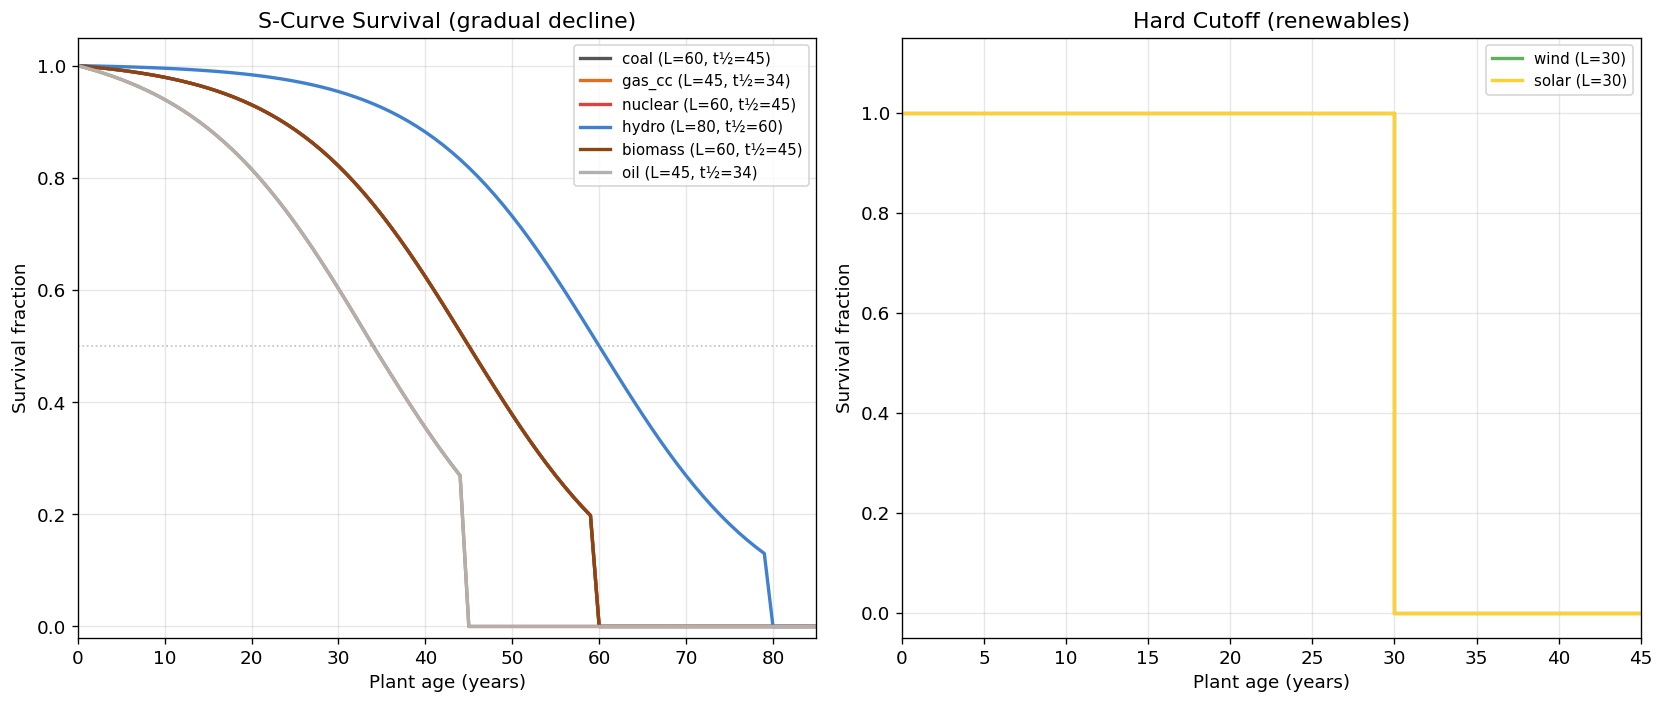
\includegraphics[width=\linewidth, height=0.82\textheight, keepaspectratio]{scurve.png}
\end{frame}

% ── Slide 18: Profit Shutdown ────────────────────────────────────
\begin{frame}{Profit Shutdown}
\centering
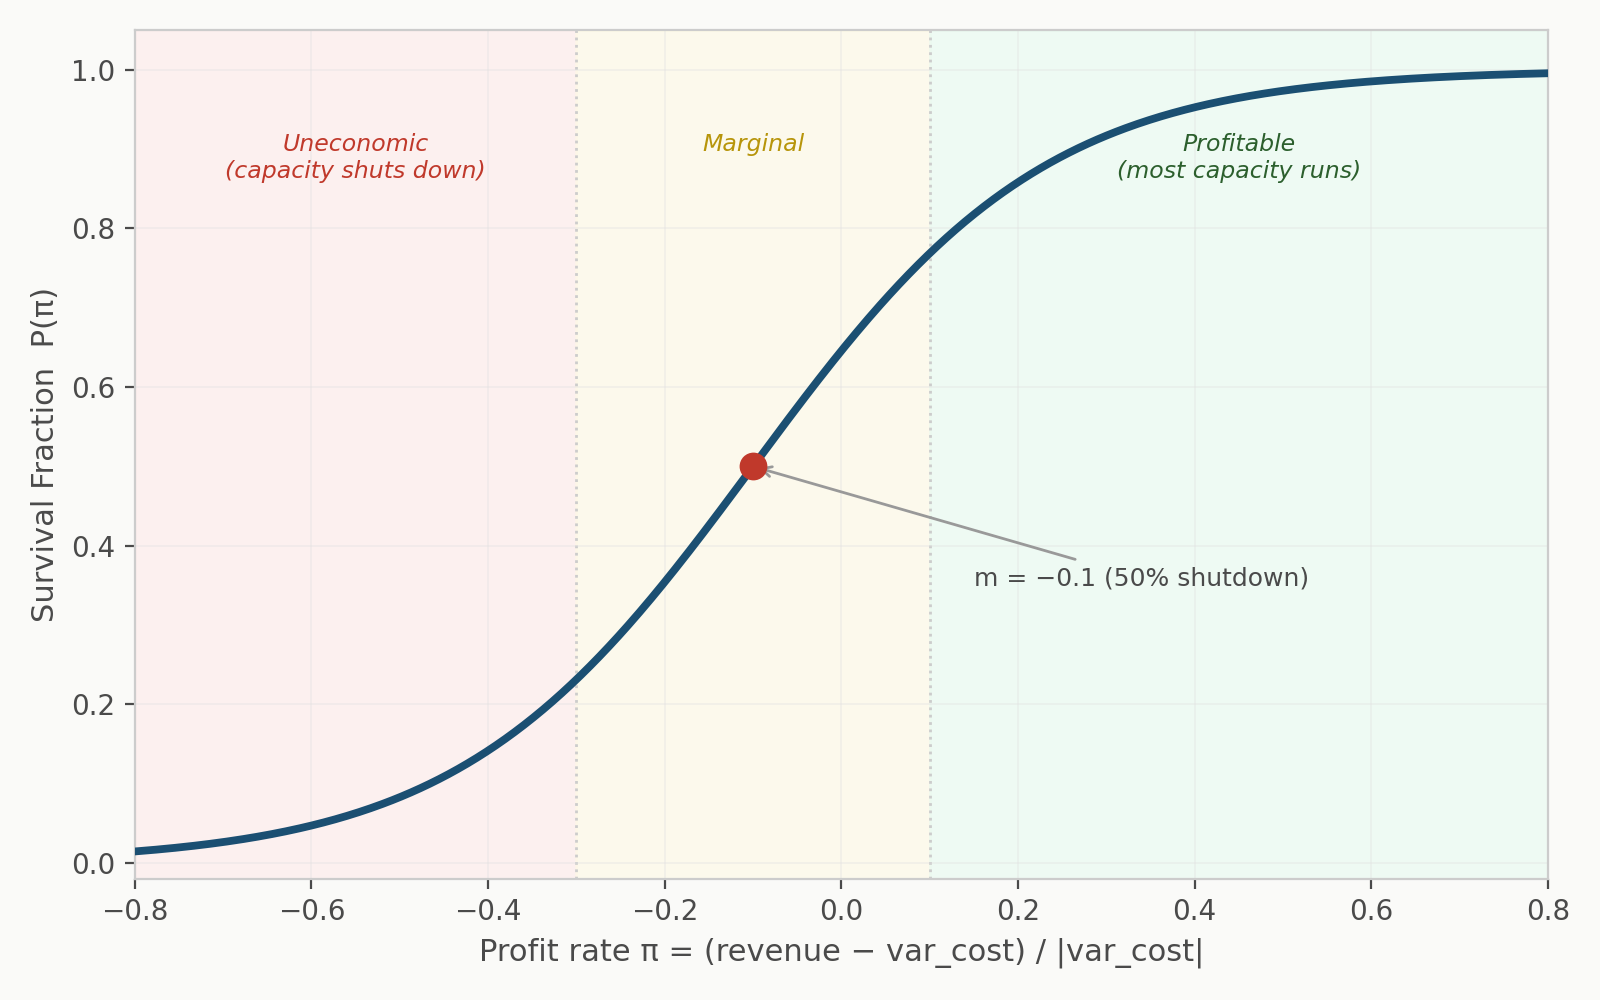
\includegraphics[width=\linewidth, height=0.82\textheight, keepaspectratio]{profit_shutdown.png}
\end{frame}

% ── Slide 19: Construction Lead Time ─────────────────────────────
\begin{frame}{Construction Lead Time}
{\small Construction time affects technology choice at two levels:}

\vspace{0.3em}
\begin{tcolorbox}[infobox, colback=green!6, colframe=green!50!black, top=2pt, bottom=2pt, title=Physical Delay]
\small
$\mathrm{gap} = \mathrm{demand} - \mathrm{surviving} - \mathrm{under\text{-}construction}$

\smallskip
\scriptsize
\bi
  \item Under-construction capacity tracked by year
  \item Nuclear: 2 periods (10yr), Hydro: 1 period (5yr)
  \item Gap-filling accounts for in-construction capacity
\ei
\end{tcolorbox}
\vspace{-0.15em}
\begin{tcolorbox}[infobox, colback=blue!6, colframe=blue!60, top=2pt, bottom=2pt, title=Interest During Construction (IDC)]
\small
$K_{\mathrm{eff}} = K_0 \times (1+r)^{T_{\mathrm{build}}}$

\smallskip
\scriptsize
\bi
  \item Capital tied up during build earns no return
  \item Nuclear (10yr, $r\!=\!8\%$): $2.16\times$ capital cost
  \item Naturally discourages long-build tech in logit
\ei
\end{tcolorbox}
\end{frame}

\section{Solver}

% ── Slide: Solver Design ──────────────────────────────────────────
\begin{frame}[t]{Solver Design}
\vspace{0.1em}

\begin{columns}[T]
\column{0.48\textwidth}

\begin{tcolorbox}[infobox, colframe=SpruceGreen, colback=SpruceGreen!5,
  title={\color{white}Approach}, colbacktitle=SpruceGreen, height=6.0cm]
\footnotesize
\textbf{1.\; Recursive-dynamic}\\[2pt]
\quad Solve one period at a time (2025--2150)\\[1pt]
\quad $\mathbf{x}_{n+1} = \alpha\, F(\mathbf{x}_n) + (1\!-\!\alpha)\,\mathbf{x}_n$

\vspace{6pt}
\textbf{2.\; State vector} --- 133 Dimensions\\[2pt]
\quad Regional ($\times$32): $(Y_r,\, I_{E,r},\, p_{\mathrm{elec},r},\, p_{\mathrm{H_2},r})$\\[1pt]
\quad Global ($\times$5): $\mathbf{p}^W\!=\!(p_\mathrm{coal},\, p_\mathrm{oil},\, p_\mathrm{gas},\, p_\mathrm{bio},\, p_\mathrm{U})$

\vspace{6pt}
\textbf{3.\; Implementation}\\[2pt]
\quad $\alpha\!=\!0.3$ (adaptive)\\[1pt]
\quad tol $= 5\!\times\!10^{-3}$,\; max\_iter $= 150$\\[3pt]
\quad {\scriptsize Inline pref recalibration per $F(\mathbf{x})$ call}\\
\quad {\scriptsize Inter-period demand carry-forward ($\alpha_{ind}$)}
\end{tcolorbox}

\column{0.48\textwidth}

\begin{tcolorbox}[infobox, colframe=blue!50, colback=blue!5,
  title={\color{white}Performance}, colbacktitle=blue!60, height=6.0cm]
\small
\begin{tabular}{@{}l r@{}}
\toprule
\textbf{Phase} & \textbf{Time} \\
\midrule
\rowcolor{SpruceGreen!8}
Data loading (Parquet $\to$ \texttt{pandas}) & 0.9s \\
TFP calibration & 36s \\
{\scriptsize \quad 4 passes $\times$ 26 periods} & \\
\rowcolor{SpruceGreen!8}
Forward solve & 14s \\
{\scriptsize \quad 26 periods $\times$ $\sim$0.5s/period} & \\
{\scriptsize \quad 2 FE recal rounds + inline recal} & \\
{\scriptsize \quad per iter: $F(\mathbf{x})$ over 32 regions} & \\
\midrule
\textbf{Total} & \textbf{$\sim$50s} \\
\bottomrule
\end{tabular}

\vspace{0.3em}
{\scriptsize Single-thread Python. \textbf{26/26 periods converge.}}
\end{tcolorbox}

\end{columns}

\end{frame}

% ── Slide: Model Pass F(x) ───────────────────────────────────────
\begin{frame}[t]{Model Pass $F(\mathbf{x})$}
\vspace{0.1em}
\centering
\begin{tikzpicture}[
  step/.style={rounded corners=3pt, minimum height=1.05cm,
               align=center, font=\small\bfseries, inner sep=5pt, minimum width=5.2cm},
  num/.style={circle, fill=gray!15, font=\scriptsize\bfseries, inner sep=1.5pt,
              text=gray!70},
  arr/.style={-{Stealth[length=4pt]}, gray!50, line width=0.8pt},
  upd/.style={-{Stealth[length=3pt]}, dashed, gray!40, line width=0.6pt},
  ulbl/.style={font=\small, text=SpruceGreen!80!black, anchor=west},
  sub/.style={font=\scriptsize, text=gray!70, anchor=north west},
  scale=0.78, transform shape,
]
  \def\bw{4.6cm}
  \def\bx{6pt}
  \def\gap{0.28cm}  % uniform edge-to-edge gap

  \node[step, fill=teal!8, draw=teal!40, align=left, text width=\bw, inner xsep=\bx] (econ) at (0,0)
    {\hfil 1.\; Economy (KLEM)\hfil\\[-2pt]
     {\scriptsize\quad$\bullet$\; Aggregate energy demand}};

  \node[step, fill=blue!8, draw=blue!40, align=left, text width=\bw, inner xsep=\bx,
        below=\gap of econ] (dem)
    {\hfil 2.\; Demand Sectors\hfil\\[-2pt]
     {\scriptsize\quad$\bullet$\; Inline pref recalibration $\to$ logit}};

  \node[step, fill=violet!8, draw=violet!40, align=left, text width=\bw, inner xsep=\bx,
        below=\gap of dem] (carrier)
    {\hfil 3.\; Transformation\hfil\\[-2pt]
     {\scriptsize\quad$\bullet$\; Elec / H$_2$ + profit shutdown}};

  \node[step, fill=orange!8, draw=orange!40, align=left, text width=\bw, inner xsep=\bx,
        below=\gap of carrier] (trade)
    {\hfil 4.\; Trade Clearing\hfil\\[-2pt]
     {\scriptsize\quad$\bullet$\; $\sum_r Q^s_r(p^*) = \sum_r Q^d_r(p^*)$}};

  \node[step, fill=green!8, draw=green!40, align=left, text width=\bw, inner xsep=\bx,
        below=\gap of trade] (price)
    {\hfil 5.\; Consumer Prices\hfil\\[-2pt]
     {\scriptsize\quad$\bullet$\; Carbon-inclusive delivered prices}};

  \node[step, fill=red!8, draw=red!40, align=left, text width=\bw, inner xsep=\bx,
        below=\gap of price] (ces)
    {\hfil 6.\; GDP Update\hfil\\[-2pt]
     {\scriptsize\quad$\bullet$\; $Y' = Q' - p'_E E - p_M M$}};

  \node[step, fill=yellow!8, draw=yellow!50, align=left, text width=\bw, inner xsep=\bx,
        below=\gap of ces] (emis)
    {\hfil 7.\; Emissions\hfil\\[-2pt]
     {\scriptsize\quad$\bullet$\; CO$_2$, CH$_4$, N$_2$O, F-gases}};

  % ── Vertical flow ──
  \draw[arr] (econ) -- (dem);
  \draw[arr] (dem) -- (carrier);
  \draw[arr] (carrier) -- (trade);
  \draw[arr] (trade) -- (price);
  \draw[arr] (price) -- (ces);
  \draw[arr] (ces) -- (emis);

  % ── Right-side annotations ──
  \def\ux{4.8}
  \draw[upd] (carrier.east) -- +(\ux-2.6,0) node[ulbl] {$p'_{\mathrm{elec}},\;\; p'_{\mathrm{H_2}},\;\; I'_E$};
  \node[font=\scriptsize, text=SpruceGreen!70!black, anchor=south, fill=white, inner sep=1pt] at ($(carrier.east)!0.5!(carrier.east)+(\ux-2.6,0)+(0,0.12)$) {\textit{cost-weighted avg}};
  \draw[upd] (trade.east) -- +(\ux-2.6,0) node[ulbl] {$p'^{W}_{\mathrm{coal}},\; p'^{W}_{\mathrm{oil}},\; p'^{W}_{\mathrm{gas}},\; p'^{W}_{\mathrm{bio}},\; p'^{W}_{\mathrm{U}}$};
  \node[font=\scriptsize, text=SpruceGreen!70!black, anchor=south, fill=white, inner sep=1pt] at ($(trade.east)!0.5!(trade.east)+(\ux-2.6,0)+(0,0.12)$) {\textit{bisection ($<$50 iter)}};
  \draw[upd] (ces.east) -- +(\ux-2.6,0) node[ulbl] {$Y'$};
  % Emissions: no state vector update (accounting only)

  % ── Feedback arrow: 7 west → up → 1 west ──
  \coordinate (midpt) at ($(econ.west)!0.5!(emis.west) + (-4.3,0)$);
  \draw[{Stealth[length=6pt]}-, SpruceGreen, line width=1.2pt, dashed]
    (econ.west) -- (econ.west -| midpt) -- (emis.west -| midpt) -- (emis.west);
  \node[fill=SpruceGreen!8, draw=SpruceGreen, rounded corners=2pt,
        font=\small\bfseries, inner sep=4pt, text=SpruceGreen!80!black]
    at (midpt) {$\mathbf{x}' \!=\! F(\mathbf{x})$};
\end{tikzpicture}
\end{frame}

\section{Results \& Next Steps}

% ── Val 1: GDP ───────────────────────────────────────────────────
\begin{frame}[t]{Calibration --- GDP \& Population}
\vspace{-0.3em}
{\small
\bi[leftmargin=1.2em, itemsep=1pt, topsep=0pt]
\item \textbf{GDP}: CC\,=\,1.0000, MAE\,=\,0.3\,B\$ --- TFP reproduces GCAM GDP trajectories
\item \textbf{Population}: SSP demographic projections applied per R32 region
\ei}
\vspace{0.1em}

\centering
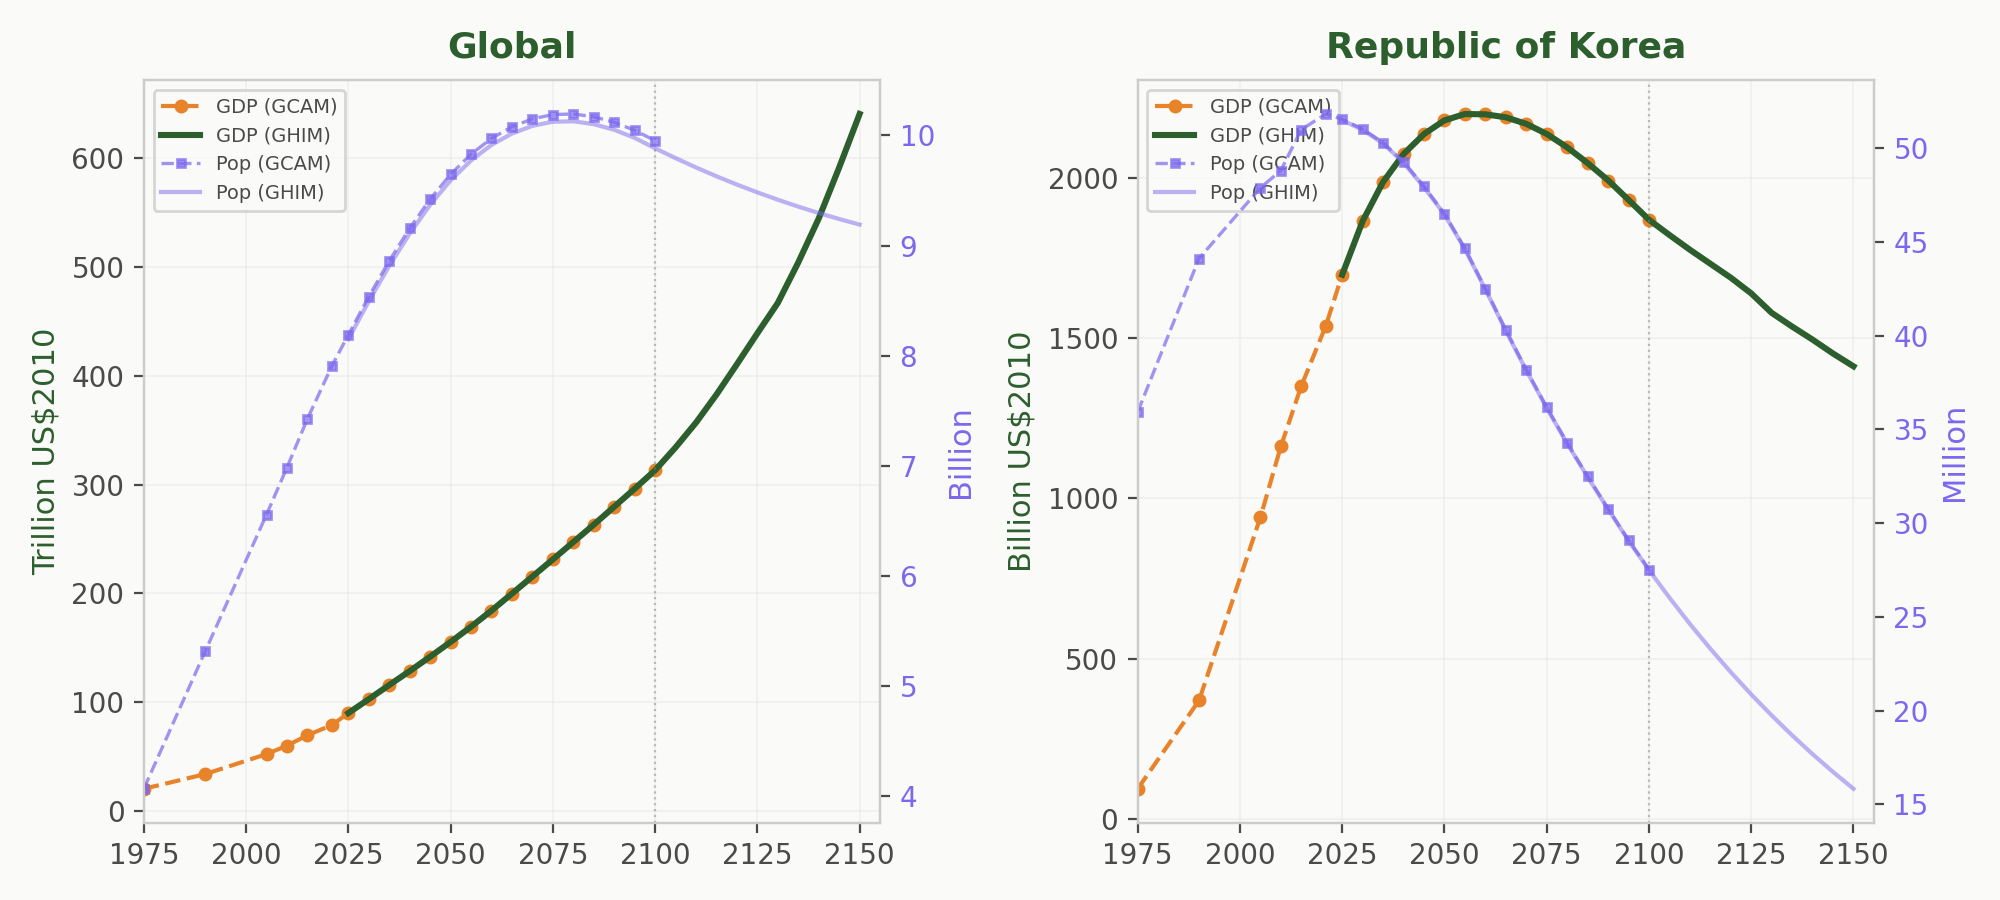
\includegraphics[width=\linewidth, height=0.76\textheight, keepaspectratio]{val_gdp_2p.png}
\end{frame}

% ── Val 2: FE by Sector ─────────────────────────────────────────
\begin{frame}[t]{Calibration --- Final Energy by Sector}
\vspace{-0.3em}
{\small \textbf{FE}: All sectors $\pm$1\% (2025--2100). Post-2100: endogenous projection with TFP extrapolation.}
\vspace{0.2em}

\centering
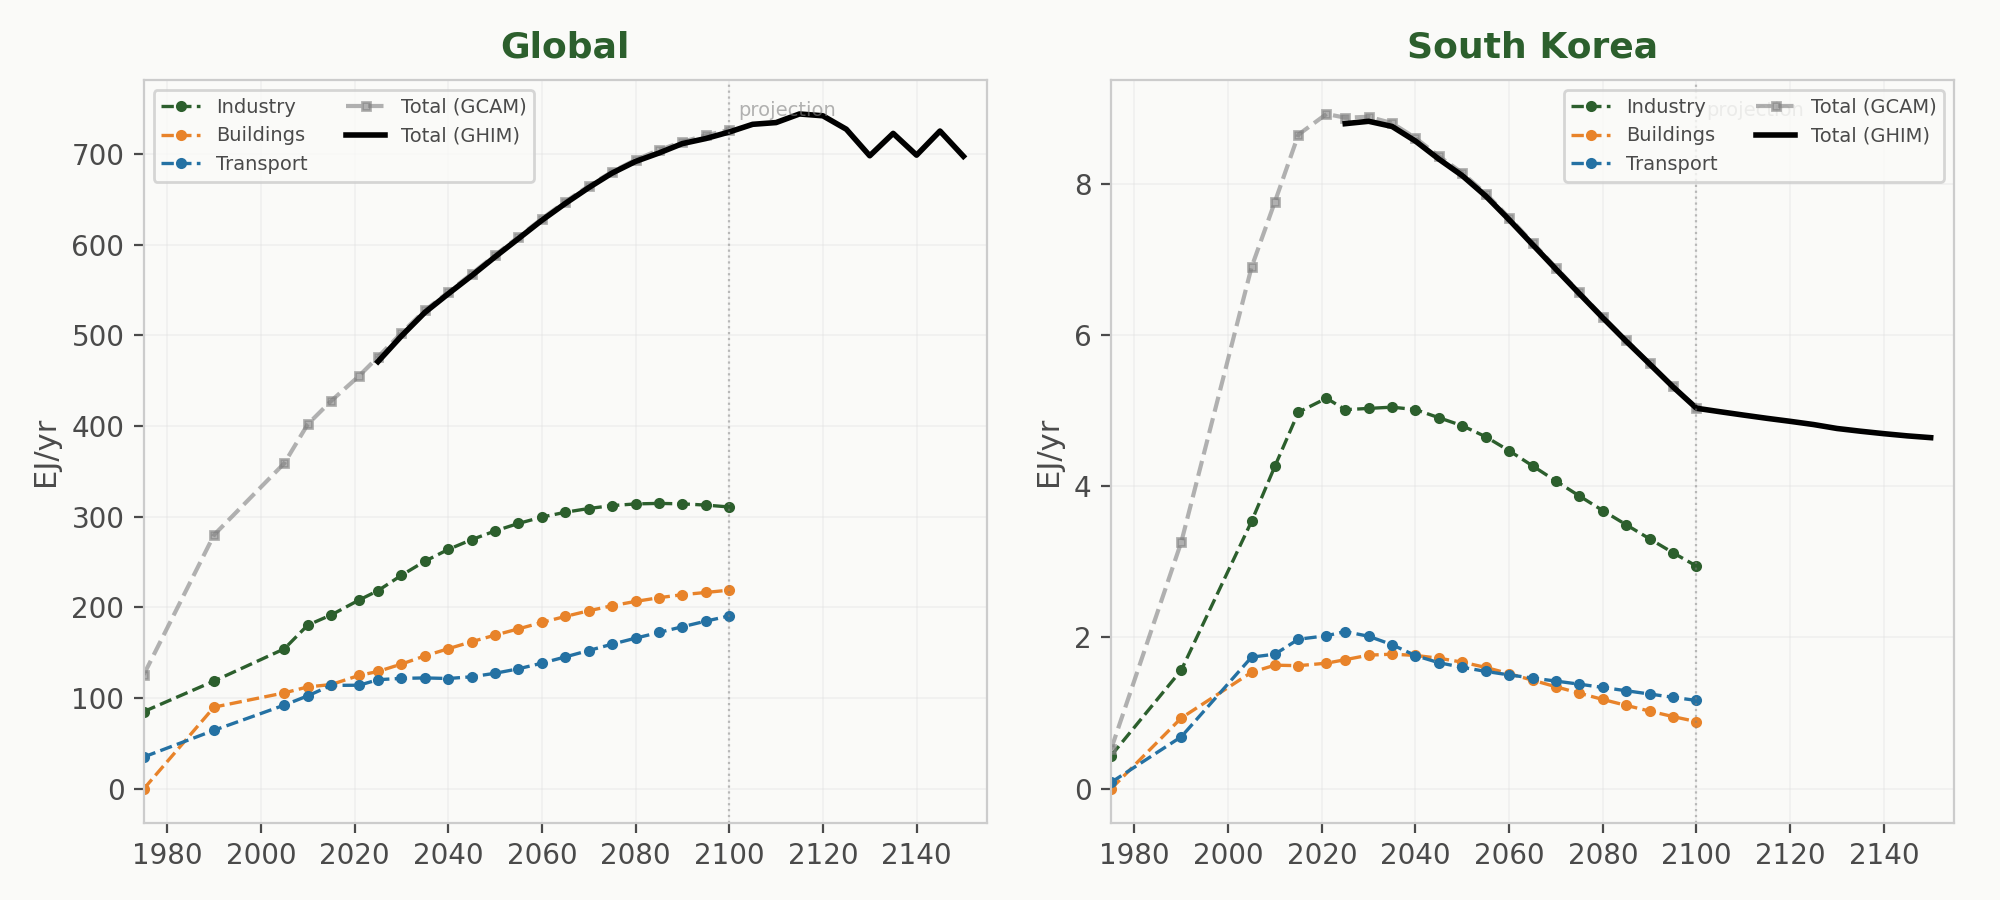
\includegraphics[width=\linewidth, height=0.82\textheight, keepaspectratio]{val_fe_sector_2p.png}
\end{frame}

% ── Val 3: FE by Carrier ────────────────────────────────────────
\begin{frame}[t]{Calibration --- Final Energy by Carrier}
\vspace{-0.3em}
{\small Carrier share trajectories --- dashed\,=\,GCAM, solid\,=\,GHIM. All carriers $\pm$2.7\,EJ.}
\vspace{0.2em}

\centering
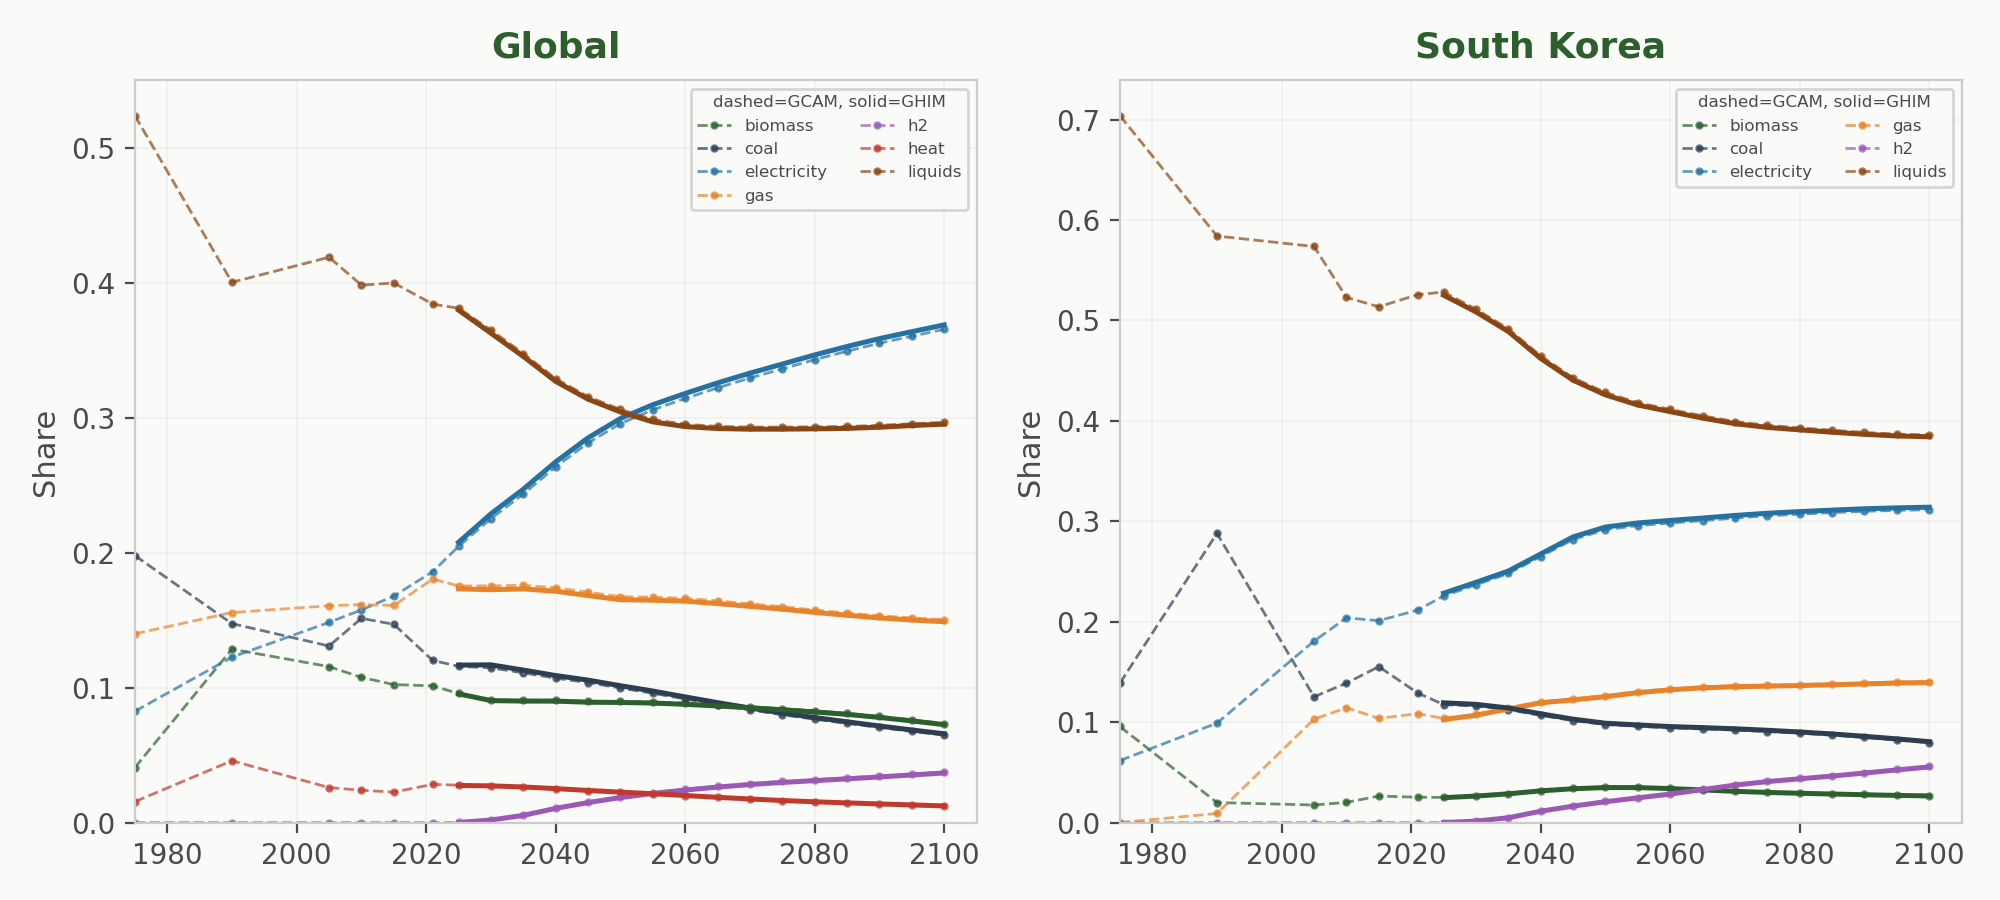
\includegraphics[width=\linewidth, height=0.82\textheight, keepaspectratio]{val_fe_carrier_2p.png}
\end{frame}

% ── Val 4: Electricity Generation (2-panel) ──────────────────────
\begin{frame}[t]{Calibration --- Electricity Generation}
\vspace{-0.3em}
{\small \textbf{Elec gen: CC\,=\,1.0000, 0.0\% deviation all periods.} H$_2$: 0.0\%. District heat: 0.0\%.}
\vspace{0.2em}

\centering
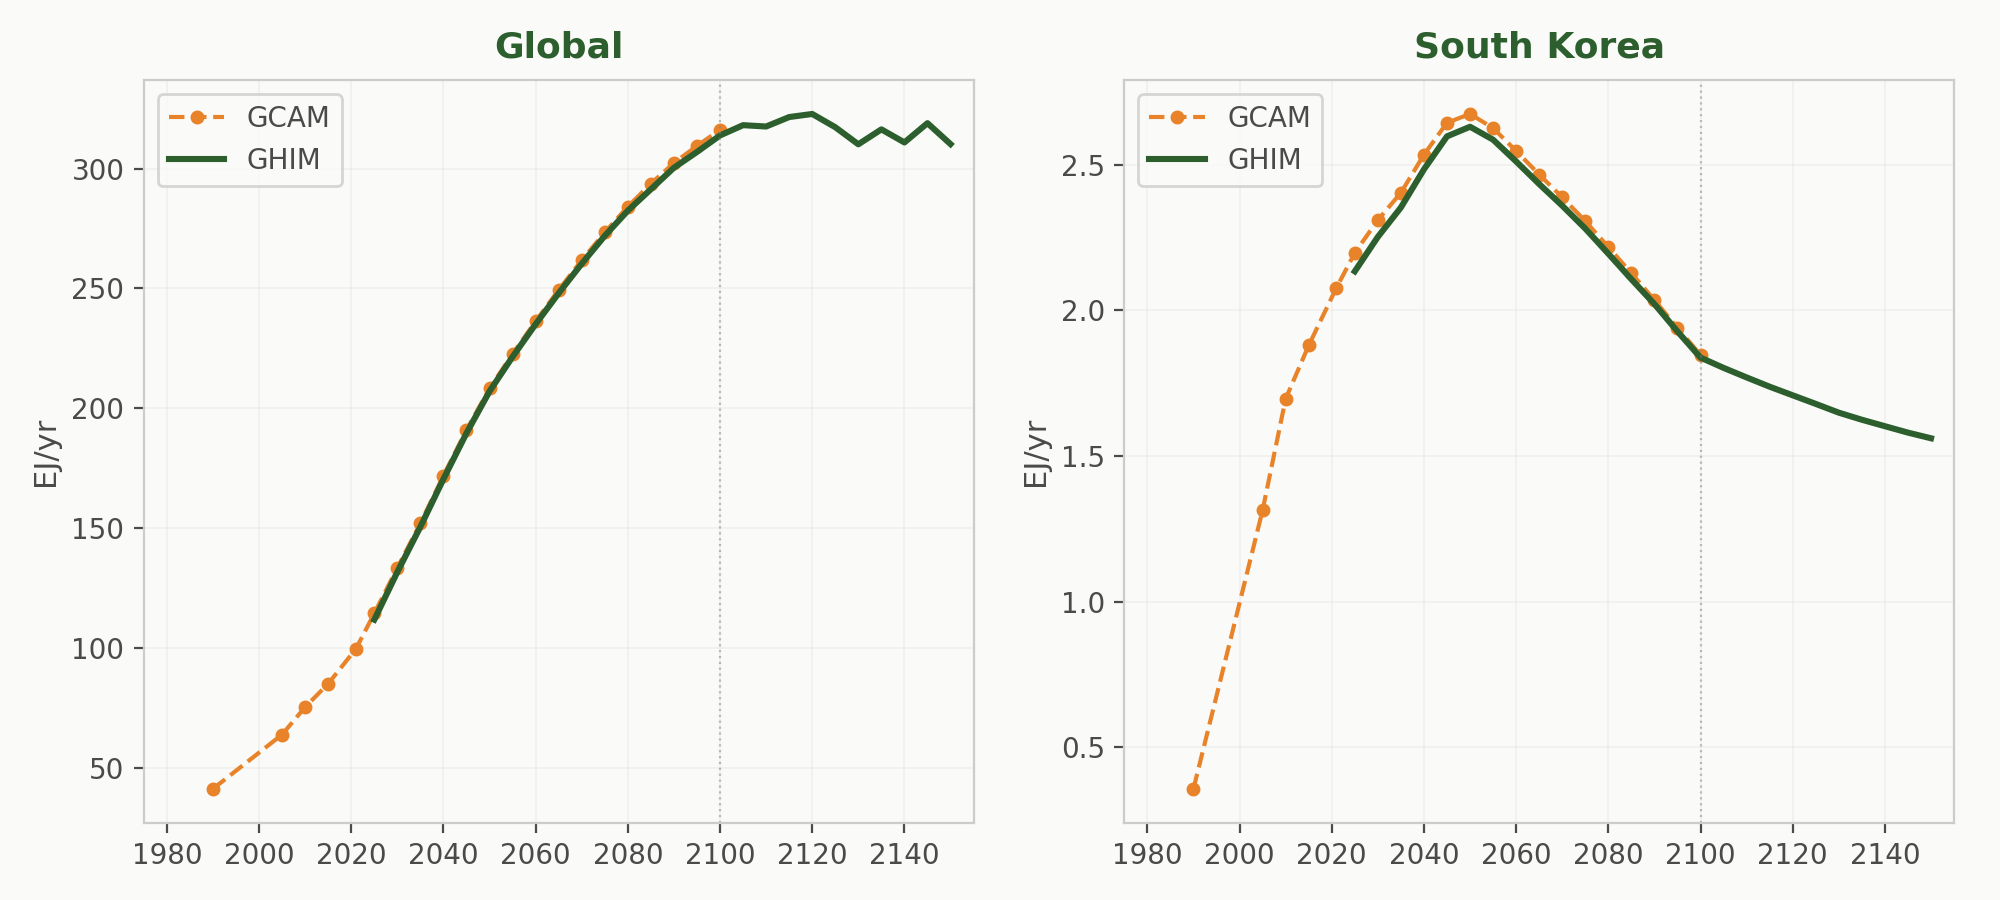
\includegraphics[width=\linewidth, height=0.82\textheight, keepaspectratio]{val_elec_gen_2p.png}
\end{frame}

% ── Val 5: Electricity Mix (2-panel) ────────────────────────────
\begin{frame}[t]{Calibration --- Electricity Generation Mix}
\vspace{-0.3em}
{\small Generation technology shares --- dashed\,=\,GCAM, solid\,=\,GHIM. All techs $\pm$1\,pp.}
\vspace{0.2em}

\centering
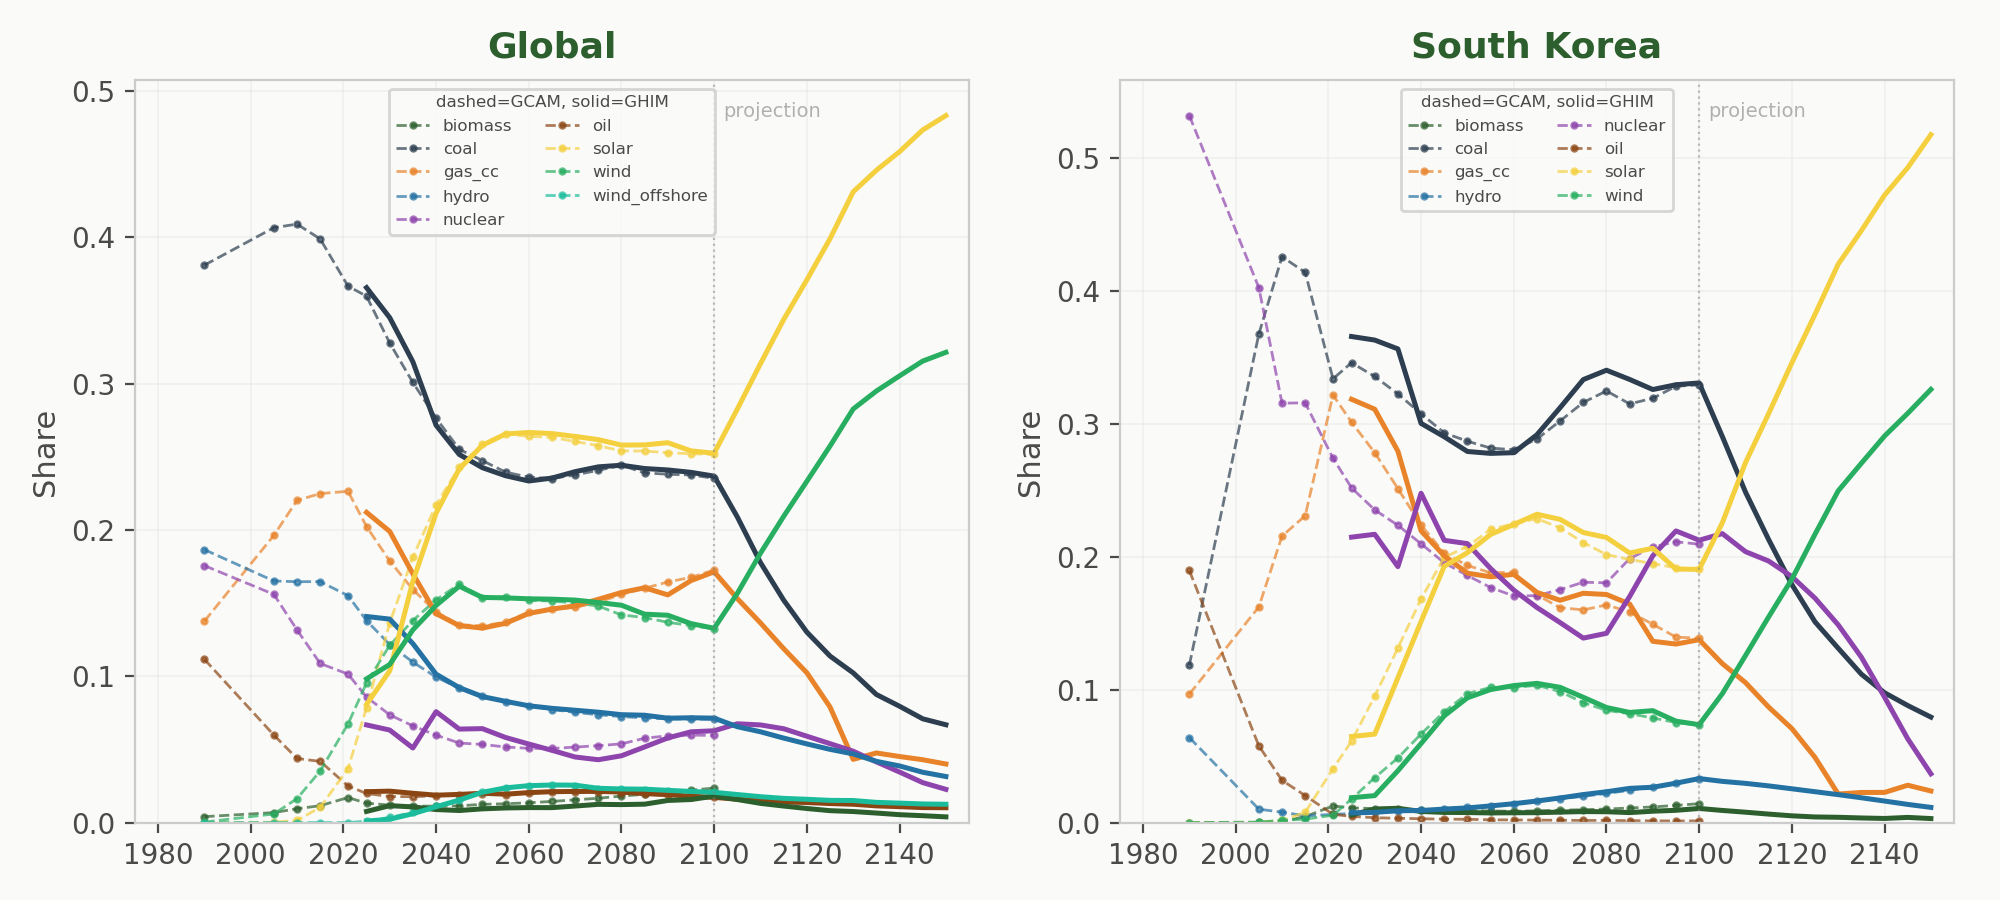
\includegraphics[width=\linewidth, height=0.82\textheight, keepaspectratio]{val_elec_mix_2p.png}
\end{frame}

% ── Slide: Next Steps ────────────────────────────────────────────
\begin{frame}{Next Steps}
\centering
\footnotesize
\begin{tabular}{l p{5.8cm} p{5.8cm}}
\toprule
\textbf{Component} & \textbf{Phase 1} & \textbf{Phase 2} \\
\midrule
\rowcolor{SpruceGreen!8}
Time          & 2000--2150, 5-year steps              & Annual resolution \\
Region        & 32 Regions                 & 100+ countries \\
\rowcolor{SpruceGreen!8}
Economy       & GDP $= f$(Capital, Labor, Energy, Materials) & + Energy intensity $EI = f(\mathrm{RND})$ \\
Solution      & Recursive-dynamic                      & Adjustable rolling foresight \\
\rowcolor{SpruceGreen!8}
Energy System & Minimum nesting for AR6 Tier-1         & Expanded nesting for Tier-3 \\
Trade         & Global fossil fuel market clearing      & Multi-commodity global trade \\
Coupling      & One-way coupling with Land              & Two-way with multiple modules \\
\midrule
\rowcolor{SpruceGreen!8}
\multicolumn{1}{l}{Tech.\ Choice} & \multicolumn{2}{p{10.0cm}}{Absolute cost logit with SSP-calibrated preference weights} \\
\multicolumn{1}{l}{Tech.\ Change} & \multicolumn{2}{p{10.0cm}}{Two-factor learning: RND knowledge + cumulative deployment (LBD)} \\
\bottomrule
\end{tabular}
\end{frame}

% ── Slide: Thank You ─────────────────────────────────────────────
\begin{frame}[plain,c]
\centering
{\Huge\color{SpruceGreen}\textbf{Thank You}}

\vspace{1.5em}
{\large\color{gray} Questions \& Discussion}
\end{frame}


% ══════════════════════════════════════════════════════════════════
% APPENDIX — slides after this point are not counted in the main
% slide numbering.  Move detailed / backup slides here.
% ══════════════════════════════════════════════════════════════════
\appendix

\section{Appendix}

% ── Original detailed Motivation table ───────────────────────────
\begin{frame}{Motivation: What GHIM Brings (Detailed)}
\vspace{0.3em}
\centering
\scriptsize
\begin{tabular}{@{} l l l @{}}
\toprule
& \textbf{Before} & \textbf{GHIM} \\
\midrule
\rowcolor{blue!6}
\textbf{\color{blue!60}Economy}
  & \begin{tabular}[t]{@{}l@{}} $\cdot$ More energy detail, less macro feedback \\ $\cdot$ Coupled models often soft-linked \end{tabular}
  & \begin{tabular}[t]{@{}l@{}} $\cdot$ Energy $\leftrightarrow$ production feedback (KLEM) \\ $\cdot$ Energy investment crowds out capital \\ $\cdot$ Consistent capital, energy, materials accounting \end{tabular} \\[4pt]
\textbf{\color{red!60!black}Climate}
  & \begin{tabular}[t]{@{}l@{}} $\cdot$ Soft coupling or offline \\ $\cdot$ Mostly through damage function \\ $\cdot$ Often one-sided \end{tabular}
  & \begin{tabular}[t]{@{}l@{}} $\cdot$ Same-period hard coupling \\ $\cdot$ Climate $\to$ Economy: multiple channels \\ \quad {\tiny -- TFP damage} \\ \quad {\tiny -- Physical: efficiency, resources, demand} \\ $\cdot$ Energy $\to$ Climate via emissions \end{tabular} \\[4pt]
\rowcolor{purple!6}
\textbf{\color{purple!60}Technology}
  & \begin{tabular}[t]{@{}l@{}} $\cdot$ Mostly fixed cost assumptions \\ $\cdot$ Exception: WITCH (optimized RND) \end{tabular}
  & \begin{tabular}[t]{@{}l@{}} $\cdot$ Two-factor learning (RND + LBD) \\ $\cdot$ Global spillovers across technology families \\ $\cdot$ Energy investment reduces available capital \end{tabular} \\[4pt]
\textbf{\color{orange!70!black}Foresight}
  & Myopic or perfect foresight
  & Adjustable rolling horizon \\[4pt]
\rowcolor{green!6}
\textbf{\color{green!50!black}Resolution \& Nesting}
  & \begin{tabular}[t]{@{}l@{}} $\cdot$ $\sim$32 regions, 5-year timesteps \\ $\cdot$ Theoretically flexible \\ $\cdot$ Hard to customize in practice \end{tabular}
  & \begin{tabular}[t]{@{}l@{}} $\cdot$ 100+ countries, annual resolution \\ $\cdot$ User-configurable sector nesting \end{tabular} \\[4pt]
\rowcolor{cyan!6}
\textbf{\color{cyan!60!black}Reporting}
  & \begin{tabular}[t]{@{}l@{}} $\cdot$ Post-hoc translation for IPCC \\ $\cdot$ Custom reporting possible but rarely used \end{tabular}
  & \begin{tabular}[t]{@{}l@{}} $\cdot$ Direct AR6 IAMC-format output \\ $\cdot$ Flexible reporting with user-defined functions \end{tabular} \\
\bottomrule
\end{tabular}
\end{frame}


% ══════════════════════════════════════════════════════════════════
% Formal Calibration — 4 backup slides
% ══════════════════════════════════════════════════════════════════

% ── (1/5) CES Nesting & Share Parameters ─────────────────────────
\begin{frame}[t]{Formal Calibration (1/4): CES Nesting \& Share Parameters}
\vspace{-0.3em}

\begin{tcolorbox}[enhanced, colback=gray!3, colframe=gray!50, top=4pt, bottom=4pt, fonttitle=\small\bfseries, title=4-Level Nested CES Production Function]
\footnotesize
\begin{tabular}{@{}llll@{}}
\textbf{Level 1} & $\mathrm{KL} = A \cdot \mathrm{CES}(K,\, L;\; \sigma_{KL}\!=\!0.8)$
  & & Capital--Labor \quad ($A$ = productivity) \\[3pt]
\textbf{Level 2} & $E_{\mathrm{val}} = \mathrm{CES}(E_{\mathrm{EL}},\, E_{\mathrm{NEL}};\; \sigma_{E}\!=\!2.0)$
  & & Electricity--Non-elec \\[3pt]
\textbf{Level 3} & $\mathrm{KLE} = \varphi_{\mathrm{KLE}} \cdot \mathrm{CES}(\mathrm{VA},\, E_{\mathrm{val}};\; \sigma_{KLE}\!=\!0.4)$
  & & Value-added--Energy \\[3pt]
\textbf{Level 4} & $Q = \varphi_{\mathrm{KLEM}} \cdot \mathrm{CES}(\mathrm{KLE},\, M;\; \sigma_{KLEM}\!=\!0.2)$
  & & Gross output \\
\end{tabular}
\end{tcolorbox}

\vspace{0.2em}
\begin{tcolorbox}[infobox, colback=green!6, colframe=green!50!black, top=4pt, bottom=4pt, title={Share Parameters $\alpha_i$ (base year, time-invariant)}]
\footnotesize
At each nest, $\alpha_i$ is calibrated from base-year cost shares:
\[
s_i = \frac{p_i \cdot X_i}{\sum_j p_j \cdot X_j}
\qquad\Longrightarrow\qquad
\alpha_i = \frac{s_i \cdot p_i^{\,\sigma-1}}{\sum_j s_j \cdot p_j^{\,\sigma-1}}
\]
\vspace{-0.8em}

KL nest: $K$, $L$ are factor stocks, so factor prices $r$, $w$ imputed from income shares ($\alpha_K\!=\!0.3$).\\
All other nests: inputs already in value terms (billion \$), so $p_i\!\cdot\! X_i$ computed directly from data.
\end{tcolorbox}

\end{frame}

% ── (2/5) Scale Factors ──────────────────────────────────────────
\begin{frame}[t]{Formal Calibration (2/4): Normalization Constants $\varphi$}
\vspace{-0.3em}

\begin{tcolorbox}[infobox, colback=blue!6, colframe=blue!60, top=4pt, bottom=4pt, title={Normalization Constants $\varphi$ (base year, time-invariant)}]
\footnotesize
Each nest gets a constant so CES output matches observed base-year values:
\begin{align*}
\varphi_{\mathrm{KLE}} &= \mathrm{KLE}_0 \;/\; \mathrm{CES}(\mathrm{VA}_0,\, E_{\mathrm{val},0})
  & \text{where } \mathrm{KLE}_0 &= \mathrm{GDP}_0 + p_E \!\cdot\! E_0 \\[4pt]
\varphi_{\mathrm{KLEM}} &= Q_0 \;/\; \mathrm{CES}(\mathrm{KLE}_0,\, M_0)
  & \text{where } Q_0 &= \frac{\mathrm{GDP}_0 + p_E \!\cdot\! E_0}{1 - m}
\end{align*}
\end{tcolorbox}

\vspace{0.3em}
\begin{tcolorbox}[enhanced, colback=gray!3, colframe=gray!50, top=4pt, bottom=4pt, fonttitle=\small\bfseries, title=Base-year input computation]
\footnotesize
\begin{itemize}[nosep,leftmargin=*,itemsep=4pt]
\item $E_{\mathrm{val},0} = p_E \!\cdot\! E_0$: energy expenditure ($p_E$ = expenditure-weighted avg of carrier prices, currently global)
\item $\mathrm{VA}_0 = \mathrm{GDP}_0 = r\!\cdot\! K + w\!\cdot\! L$: factor income, enforced by $A$ calibration
\item $\mathrm{KLE}_0 = \mathrm{GDP}_0 + E_{\mathrm{val},0}$: value-added \textbf{plus} energy cost
\item $M_0 = m \cdot Q_0$,\quad $Q_0 = \mathrm{KLE}_0 \,/\, (1\!-\!m)$\quad ($m = 0.45$, materials share)
\end{itemize}
\end{tcolorbox}

\end{frame}

% ── (3/5) Base-Year TFP ──────────────────────────────────────────
\begin{frame}[t]{Formal Calibration (3/4): Base-Year Productivity $A_0$}
\vspace{-0.3em}

\begin{tcolorbox}[infobox, colback=orange!6, colframe=orange!70!black, top=4pt, bottom=4pt, title={Base-Year Productivity $A_0$ (iterative calibration)}]
\footnotesize
Find $A_0$ such that $\mathrm{GDP} = Q - p_E\!\cdot\! E - m\!\cdot\! Q = \mathrm{GDP}_0$:

\begin{align*}
&\text{Initial guess: } A = \mathrm{GDP}_0 \,/\, \mathrm{CES}_{KL}(K_0,\, L_0) \\[6pt]
&\textbf{repeat:} \\
&\quad \mathrm{VA} = A \cdot \mathrm{CES}_{KL}(K_0,\, L_0) \\
&\quad E = E_0 \cdot \mathrm{VA}\,/\,\mathrm{VA}_0
  \qquad\text{\small(price ratio = 1 at base year)} \\
&\quad \mathrm{GDP}_{\mathrm{out}} = Q(\mathrm{VA},\, E) - p_E\!\cdot\! E - m\!\cdot\! Q \\
&\quad A \leftarrow A \times \mathrm{GDP}_0 \,/\, \mathrm{GDP}_{\mathrm{out}} \\[4pt]
&\textbf{until } |\mathrm{GDP}_{\mathrm{out}} - \mathrm{GDP}_0| \,/\, \mathrm{GDP}_0 < 10^{-10}
\end{align*}
\end{tcolorbox}

\vspace{0.3em}
\begin{tcolorbox}[enhanced, colback=gray!3, colframe=gray!50, top=4pt, bottom=4pt, fonttitle=\small\bfseries, title=Notes]
\footnotesize
\begin{itemize}[nosep,leftmargin=*,itemsep=4pt]
\item Converges in 3--5 iterations (Newton-like ratio correction)
\item At base year, energy price $= p_{E,0}$, so $E \propto \mathrm{VA}$ (no price effect)
\item $A_0$ ensures the full chain KL $\!\to\!$ KLE $\!\to\!$ Q $\!\to\!$ GDP reproduces GDP$_0$ exactly
\end{itemize}
\end{tcolorbox}

\end{frame}

% ── (4/5) Future TFP Trajectory ──────────────────────────────────
\begin{frame}[t]{Formal Calibration (4/4): Future Productivity $A(t)$}
\vspace{-0.3em}

\begin{tcolorbox}[infobox, colback=orange!6, colframe=orange!70!black, top=4pt, bottom=4pt, title={$A(t)$ via Bisection (every 5-year period)}]
\footnotesize
Given: $K(t)$ from capital accumulation, $L(t)$ from SSP population,
$p_E(t)$ from calibration pass.

\begin{align*}
\mathrm{VA}(t) &= A(t) \cdot \mathrm{CES}_{KL}\!\big(K(t),\, L(t)\big) \\[4pt]
E(t) &= E_0 \cdot \frac{\mathrm{VA}(t)}{\mathrm{VA}_0} \cdot \left(\frac{p_E(t)}{p_{E,0}}\right)^{\!-\sigma_{KLE}}
  \qquad\text{\small(CES first-order condition)} \\[4pt]
\mathrm{GDP}(t) &= Q\!\big(\mathrm{VA}(t),\, E(t)\big) - p_E(t)\!\cdot\! E(t) - m\!\cdot\! Q
\end{align*}

\vspace{-0.5em}
Bisect $A(t)$ until $\mathrm{GDP}(t) = \mathrm{GDP}_{\mathrm{SSP}}(t)$
\quad(80 iterations, tol $< 10^{-10}$).
\end{tcolorbox}

\vspace{0.3em}
\begin{tcolorbox}[enhanced, colback=gray!3, colframe=gray!50, top=4pt, bottom=4pt, fonttitle=\small\bfseries, title=Capital evolution between periods]
\footnotesize
\[
K(t+\Delta) = (1-\delta)^{\Delta}\, K(t) \;+\; s \cdot Y_{\mathrm{SSP}}(t) \cdot \Delta
\]
\vspace{-0.5em}
\begin{itemize}[nosep,leftmargin=*,itemsep=3pt]
\item $\delta = 5\%$ (depreciation),\quad $s = 22\%$ (savings rate),\quad $\Delta = 5$ years
\item $K(t)$ is computed \textbf{before} TFP bisection at each period
\item Investment uses SSP GDP (or endogenous GDP in later calibration passes)
\end{itemize}
\end{tcolorbox}

\end{frame}

% ══════════════════════════════════════════════════════════════════
% AR6 Preference Calibration — 3 backup slides
% ══════════════════════════════════════════════════════════════════

% ── (1/3) Electricity Technology Preferences ─────────────────────
\begin{frame}[t]{AR6 Preference Calibration (1/3): Electricity Technology Shares}
\vspace{-0.5em}
\scriptsize

AR6 SSP baselines specify generation shares per technology per period.
Invert the logit to recover preference factors $P_i(t)$ that reproduce these shares.

\vspace{0.2em}
\begin{tcolorbox}[infobox, colback=purple!6, colframe=purple!60, top=3pt, bottom=3pt, title={Relative Preference Logit (MERGE-style)}]
\scriptsize
\vspace{-0.5em}
\[
S_i = \frac{e^{\,\beta \cdot C_i^{\,k} + P_i}}
  {\textstyle\sum_j e^{\,\beta \cdot C_j^{\,k} + P_j}}
\]
\vspace{-1.2em}
\begin{itemize}[nosep,leftmargin=*,itemsep=2pt]
\item $S_i$: generation share,\quad $C_i$: LCOE (\$/GJ, incl.\ capital, O\&M, fuel, carbon)
\item $\beta = -4.0$: cost sensitivity,\quad $k = 0.3$: logit scale
\item $P_i$: preference factor (unknown to calibrate)
\end{itemize}
\end{tcolorbox}

\vspace{0.15em}
\begin{tcolorbox}[infobox, colback=purple!6, colframe=purple!60, top=3pt, bottom=3pt, title={Logit Inversion (every period, per R32 region)}]
\scriptsize
Reference tech $r$ = largest AR6 share, set $P_r = 0$. For each $i \neq r$:
\vspace{-0.5em}
\[
P_i = \frac{\beta}{k}\,\ln\!\left(\frac{C_i}{C_r}\right)
  - \frac{1}{k}\,\ln\!\left(\frac{S_i^{\mathrm{AR6}}}{S_r^{\mathrm{AR6}}}\right)
\]
\vspace{-1.2em}
Applied to all 17 electricity technologies per R32 region.
Roundtrip verified: calibrated preferences reproduce AR6 shares within tolerance.
\end{tcolorbox}

\end{frame}

% ── (2/3) Demand Sector Carrier Preferences ──────────────────────
\begin{frame}[t]{AR6 Preference Calibration (2/3): Demand Carrier Shares}
\vspace{-0.5em}
\scriptsize

Calibrate demand-side preferences from AR6 carrier shares (R5 data, applied per R32).

\vspace{0.1em}
\begin{tcolorbox}[infobox, colback=purple!6, colframe=purple!60, top=2pt, bottom=2pt, title={Step A: Extract AR6 Carrier Shares}]
\scriptsize
\textbf{Transport}: direct AR6 variables (3 carriers: liquids, electricity, gas).
\textbf{Industry \& Buildings}: residual method (subtract transport to avoid liquids bias):
\vspace{-0.5em}
\[
\text{share}_c^{\mathrm{ind+bld}} = (\mathrm{FE}_c^{\mathrm{total}} - \mathrm{FE}_c^{\mathrm{transport}})
  \;/\; (\mathrm{FE}^{\mathrm{total}} - \mathrm{FE}^{\mathrm{transport}})
\]
\vspace{-1.2em}
\end{tcolorbox}

\vspace{0.1em}
\begin{tcolorbox}[infobox, colback=purple!6, colframe=purple!60, top=2pt, bottom=2pt, title={Step B: Within-Carrier Tech Splitting}]
\scriptsize
Multiple techs can share one carrier (e.g., ICE and HEV both use liquids).
Split by within-carrier cost competition:
\vspace{-0.5em}
\[
S_i^{\mathrm{tech}} = S_c^{\mathrm{carrier}} \times
  e^{-k C_i}\,/\,{\textstyle\sum_{j \in c}\, e^{-k C_j}}
\]
\vspace{-1.2em}
\end{tcolorbox}

\vspace{0.1em}
\begin{tcolorbox}[infobox, colback=purple!6, colframe=purple!60, top=2pt, bottom=2pt, title={Step C: Absolute Preference Logit Inversion}]
\scriptsize
Demand sectors use absolute preference logit (no cost exponent):
\vspace{-0.5em}
\[
P_i = (C_r - C_i) - \frac{1}{k}\,\ln\!\left(\frac{S_i^{\mathrm{tech}}}{S_r^{\mathrm{tech}}}\right)
\]
\vspace{-1.2em}
Per subsector: industry, buildings, transport. Reference $r$ = largest-share tech, $P_r = 0$.
\end{tcolorbox}

\end{frame}

% ── (3/3) FE Level Scaling ───────────────────────────────────────
\begin{frame}[t]{AR6 Preference Calibration (3/3): Final Energy Level Scaling}
\vspace{-0.5em}
\scriptsize

Shares are correct, but total FE level may not match AR6 (prices change during solving).

\vspace{0.1em}
\begin{tcolorbox}[infobox, colback=purple!6, colframe=purple!60, top=3pt, bottom=3pt, title={Demand Scale Factor $\lambda_s(t)$}]
\scriptsize
Per-sector multiplicative correction to match AR6 total FE:
\vspace{-0.3em}
\[
\lambda_s(t) = \mathrm{FE}_s^{\mathrm{AR6}}(t) \;/\; \mathrm{FE}_s^{\mathrm{model}}(t)
\]
\vspace{-1.2em}
\begin{itemize}[nosep,leftmargin=*,itemsep=2pt]
\item $\mathrm{FE}_s^{\mathrm{model}}$: computed at SSP GDP with $\lambda = 1$ (unscaled)
\item Applied as: $\mathrm{FE}_s = \lambda_s \times \mathrm{FE}_s^{\mathrm{base}}$
\item Shares preserved — only total level changes, not carrier mix
\end{itemize}
\end{tcolorbox}

\vspace{0.1em}
\begin{tcolorbox}[infobox, colback=purple!6, colframe=purple!60, top=3pt, bottom=3pt, title={3$\times$ Recalibration Loop per Period}]
\scriptsize
\begin{itemize}[nosep,leftmargin=*,itemsep=2pt]
\item \textbf{Round 1}: Compute $\lambda_s$ from initial prices, run solver
\item \textbf{Round 2}: Recompute $\lambda_s$ at converged prices, re-solve
\item \textbf{Round 3}: Final check, solver re-converges
\end{itemize}
\vspace{0.15em}
Each round anchored to SSP GDP. $\lambda_s$ stabilizes within $\pm 1\%$ after round 2.
\end{tcolorbox}

\vspace{0.1em}
\begin{tcolorbox}[enhanced, colback=SpruceGreen!6, colframe=SpruceGreen, boxrule=0.8pt, arc=3pt, left=5pt, right=5pt, top=3pt, bottom=3pt, fonttitle=\scriptsize\bfseries, title=R5 to R32 downscaling]
\scriptsize
AR6 data at R5 (5 regions). Downscale to R32 via GDP share:
$\mathrm{FE}_{r32} = \mathrm{FE}_{R5} \times (\mathrm{GDP}_{r32}\,/\,\mathrm{GDP}_{R5})$
\end{tcolorbox}

\end{frame}

% ── Backup: Calibration Bootstrap — Exogenous → Endogenous ───────
% ── Backup: Bootstrap (1/2) — Problem & Pass 1 ───────────────────
\begin{frame}[t,fragile]{Calibration Bootstrap (1/2): Exogenous Pass}
\vspace{-0.3em}

\begin{tcolorbox}[enhanced, colback=red!5, colframe=red!60!black, top=3pt, bottom=3pt, fonttitle=\small\bfseries, title=Problem: circular dependency]
\footnotesize
$\mathrm{TFP}(t)$ needs $p_E(t)$,\quad
$p_E(t)$ needs model run,\quad
model run needs $\mathrm{TFP}(t)$
\end{tcolorbox}

\vspace{0.3em}
\begin{tcolorbox}[enhanced, colback=gray!3, colframe=gray!60, top=6pt, bottom=6pt, left=8pt, right=8pt, fonttitle=\small\bfseries, title=Pass 1: Exogenous GDP (break the loop)]
\footnotesize
\textrm{GDP is forced to SSP; run model to discover equilibrium energy prices.}\\[4pt]
\ttfamily
model.gdp\_mode = EXOGENOUS \hfill\textrm{\footnotesize// bypass CES for GDP}\\[3pt]
\textbf{for} t in [2025, 2030, \ldots, 2100]:\\
\quad\quad solve\_equilibrium(model, t)\\
\quad\quad ref\_price[t] = record\_energy\_prices(t)\\[6pt]
%
\textrm{\footnotesize Now use those prices to calibrate TFP properly.}\\[4pt]
\textbf{for} t in [2025, 2030, \ldots, 2100]:\\
\quad\quad bisect TFP(t) such that:\\
\quad\quad\quad\quad \textrm{$Q(t) - p_E(t)\!\cdot\! E(t) - p_M\!\cdot\! M(t) = \mathrm{GDP}_{\mathrm{SSP}}(t)$}
\end{tcolorbox}

\end{frame}

% ── Backup: Bootstrap (2/2) — Endogenous Verification ────────────
\begin{frame}[t,fragile]{Calibration Bootstrap (2/2): Endogenous Verification}
\vspace{-0.3em}

\begin{tcolorbox}[enhanced, colback=gray!3, colframe=gray!60, top=6pt, bottom=6pt, left=8pt, right=8pt, fonttitle=\small\bfseries, title=Pass 2+: Endogenous GDP (verify convergence)]
\footnotesize
\textrm{CES now determines GDP. Check if it matches SSP; iterate if not.}\\[4pt]
\ttfamily
model.gdp\_mode = ENDOGENOUS \hfill\textrm{\footnotesize// CES determines GDP}\\[3pt]
\textbf{repeat}:\\
\quad\quad solve\_all\_periods(model)\\[2pt]
\quad\quad max\_dev = max\textrm{$_{\,r,t}$}
  |GDP(r,t) - GDP\textrm{$_\text{SSP}$}(r,t)| / GDP\textrm{$_\text{SSP}$}\\[2pt]
\quad\quad \textbf{if} max\_dev < 2\%: \textbf{break}\\[2pt]
\quad\quad ref\_price = record\_energy\_prices()\\
\quad\quad re\_calibrate\_tfp(ref\_price)
\end{tcolorbox}

\vspace{0.3em}
\begin{tcolorbox}[enhanced, colback=SpruceGreen!6, colframe=SpruceGreen, boxrule=0.8pt, arc=3pt, left=5pt, right=5pt, top=4pt, bottom=4pt, fonttitle=\small\bfseries, title=Result]
\footnotesize
\begin{tabular}{@{}ll@{}}
Without bootstrap (constant-price TFP): & 7--14\% GDP deviation \\
With two-pass bootstrap: & $< 0.2\%$ GDP deviation \\
\end{tabular}
\end{tcolorbox}

\end{frame}

% ══════════════════════════════════════════════════════════════════
\section{Data Processing}
% ══════════════════════════════════════════════════════════════════

% ── Slide: Data Sources & Processing Pipeline ────────────────────
\begin{frame}[t]{Data Sources \& Processing Pipeline}
\vspace{-0.3em}

\begin{columns}[T]
\column{0.46\textwidth}

\begin{tcolorbox}[infobox, colback=SpruceGreen!5, colframe=SpruceGreen!60,
  title={\small Primary Source: gcamdata (v8.2)}]
\small
\begin{tabular}{@{}lll@{}}
\toprule
\textbf{Source} & \textbf{Data} & \textbf{Ver.} \\
\midrule
\rowcolor{SpruceGreen!8}
IEA & Energy balances & 2023 \\
IIASA SSP & Scenarios & AR6 \\
\rowcolor{SpruceGreen!8}
CEDS & Emissions & 2022 \\
GTAP & Trade & v11 \\
\rowcolor{SpruceGreen!8}
NREL ATB & Tech costs & 2024 \\
UCD & Transport & 2013 \\
\rowcolor{SpruceGreen!8}
FAO & Agriculture & 2024 \\
\bottomrule
\end{tabular}

\vspace{0.3em}
{\tiny 450+ R chunks $\to$ harmonized CSV/XML}
\end{tcolorbox}

\column{0.50\textwidth}

\begin{tcolorbox}[infobox, colback=blue!5, colframe=blue!50,
  title={\small Processing Pipeline}]
\small
\textbf{1.\; GCAM BaseX Query}\\[-1pt]
{\scriptsize XML query on v8.2 SSP2-Ref database output}

\vspace{0.25em}
\textbf{2.\; Parquet Export}\\[-1pt]
{\scriptsize \texttt{national\_accounts}, \texttt{final\_energy}, \texttt{electricity\_gen}, \texttt{population}}

\vspace{0.25em}
\textbf{3.\; CalibrationDataset}\\[-1pt]
{\scriptsize R32 $\times$ 22 years (1975--2100)\\
GDP (MER 2010\$), FE (EJ), shares, subsectors\\
GCAM 1990\$ $\to$ 2010\$ ($\times$1.5114 BEA deflator)}

\vspace{0.25em}
\textbf{4.\; Model Calibration}\\[-1pt]
{\scriptsize TFP iterative 4-pass, inverse logit prefs, FE scaling}
\end{tcolorbox}

\end{columns}

\vspace{0.3em}
\centering
{\small\color{TextLight} Total: $\sim$90s (data 3.5s + TFP calibration 36s + solve 50s)}

\end{frame}

% ── Slide: Current Data Inventory ────────────────────────────────
\begin{frame}[t]{Current Data Inventory}
\vspace{-0.2em}

\centering
\small
\begin{tabular}{@{}l l l l l@{}}
\toprule
\textbf{Category} & \textbf{Source} & \textbf{Format} & \textbf{Resolution} & \textbf{Status} \\
\midrule
\rowcolor{SpruceGreen!8}
GDP, Capital, TFP & GCAM v8.2 & Parquet & R32 $\times$ 22yr & \textcolor{SpruceGreen}{\textbf{Complete}} \\
Population & GCAM v8.2 & Parquet & R32 $\times$ 22yr & \textcolor{SpruceGreen}{\textbf{Complete}} \\
\rowcolor{SpruceGreen!8}
Final Energy (sector$\times$carrier) & GCAM v8.2 & Parquet & R32 $\times$ 22yr & \textcolor{SpruceGreen}{\textbf{Complete}} \\
Electricity Gen (tech mix) & GCAM v8.2 & Parquet & R32 $\times$ 21yr & \textcolor{SpruceGreen}{\textbf{Complete}} \\
\rowcolor{SpruceGreen!8}
Factor Shares (K, L, E) & GCAM v8.2 & Parquet & R32 $\times$ 22yr & \textcolor{SpruceGreen}{\textbf{Complete}} \\
SSP Scenarios & OECD ENV & CSV.gz & Country $\times$ 5yr & \textcolor{SpruceGreen}{\textbf{Complete}} \\
\rowcolor{SpruceGreen!8}
Fossil Supply Curves & gcamdata & CSV & R32 $\times$ 7 grades & \textcolor{SpruceGreen}{\textbf{Complete}} \\
Region Mapping & gcamdata & TSV & 249 countries & \textcolor{SpruceGreen}{\textbf{Complete}} \\
\midrule
\rowcolor{orange!8}
Technology Costs & NREL ATB & CSV & Per tech & \textcolor{orange!80!black}{\textbf{Defaults}} \\
\rowcolor{red!5}
H$_2$ Production & GCAM v8.2 & --- & R32 & \textcolor{red!70!black}{Not extracted} \\
\rowcolor{red!5}
District Heat & GCAM v8.2 & --- & R32 & \textcolor{red!70!black}{Not extracted} \\
\bottomrule
\end{tabular}

\vspace{0.5em}
{\small\color{SpruceGreen} Model naming: \texttt{GHIM-\{source\}-\{scenario\}}\quad e.g.\ \texttt{GHIM-GCAM-v8.2-SSP2-Ref}}

\end{frame}

% ── Slide: Additional Data Needs ─────────────────────────────────
\begin{frame}[t]{Additional Data Needs}
\vspace{-0.3em}

\begin{columns}[T]
\column{0.46\textwidth}

\begin{tcolorbox}[infobox, colback=red!3, colframe=red!40,
  title={\small Proprietary / Purchase Required}]
\small
\textcolor{red!70!black}{\textbf{[HIGH]}} \textbf{IEA World Energy Balances}\\
{\scriptsize Country-level energy flows for direct calibration}

\vspace{0.35em}
\textcolor{orange!80!black}{\textbf{[MED]}} \textbf{IEA Energy Technology Perspectives}\\
{\scriptsize Detailed technology cost projections by region}

\vspace{0.35em}
\textcolor{orange!80!black}{\textbf{[MED]}} \textbf{GTAP Database (v11+)}\\
{\scriptsize Bilateral trade matrices for multi-sector trade}

\vspace{0.35em}
\textcolor{gray}{\textbf{[LOW]}} \textbf{BNEF / IRENA Cost Data}\\
{\scriptsize Up-to-date renewable energy cost curves}
\end{tcolorbox}

\column{0.50\textwidth}

\begin{tcolorbox}[infobox, colback=SpruceGreen!5, colframe=SpruceGreen!60,
  title={\small Open Data / Student Tasks}]
\small
\textcolor{SpruceGreen}{\textbf{[RA]}} \textbf{GCAM BaseX: H$_2$ \& Heat}\\
{\scriptsize Extract hydrogen and district heating tech mix}

\vspace{0.3em}
\textcolor{SpruceGreen}{\textbf{[RA]}} \textbf{GCAM BaseX: Refining}\\
{\scriptsize Crude-to-product conversion by region}

\vspace{0.3em}
\textcolor{SpruceGreen}{\textbf{[RA]}} \textbf{World Bank PPP Conversion}\\
{\scriptsize PPP factors for MER-PPP bridge}

\vspace{0.3em}
\textcolor{blue!60}{\textbf{[MS/PhD]}} \textbf{HDD/CDD Climate Data}\\
{\scriptsize Projected heating/cooling degree days}

\vspace{0.3em}
\textcolor{blue!60}{\textbf{[MS/PhD]}} \textbf{Transport Mode Share}\\
{\scriptsize Passenger/freight modal split by region}
\end{tcolorbox}

\end{columns}

\vspace{0.2em}
\centering
{\small\color{TextLight} Format convention: Parquet ($>$1MB) $\cdot$ CSV (mappings) $\cdot$ TSV (region classifications)}

\end{frame}

\end{document}
